\chapter{Tempo e comprimento}
\markboth{Módulo 5}{}\enlargethispage{6\baselineskip}

\vspace*{-1.5cm}

\section*{Habilidades do SAEB}

\begin{itemize}
\item Medir ou comparar perímetro ou área de figuras planas desenhadas em malha quadriculada.

\item Identificar horas em relógios analógicos ou associar horas em relógios analógicos e digitais.

\item Resolver problemas que envolvam perímetro de figuras planas.

\item Resolver problemas que envolvam área de figuras planas.
\end{itemize}

\subsection{Habilidades da BNCC}

\begin{itemize}
 \item  EF03MA22, EF03MA23.
\end{itemize}


\conteudo{
Um dia dura 24 horas.

Uma semana é composta por 7 dias.   

\begin{myquote}
Os dias da semana são:
\begin{flushleft}
\textbf{domingo, segunda-feira, terça-feira, quarta-feira, quinta-feira, sexta-feira e sábado.}
\end{flushleft}
\end{myquote}

Um ano é composto por 12 meses. O nome dos meses e suas respectivas quantidades de dias estão na tabela a seguir.

\pagebreak

\begin{myquote}
\begin{small}
\begin{longtable}[]{@{}ll@{}}
\toprule
\textbf{Meses que compõem o ano} & \textbf{Número de dias dos meses}\tabularnewline
\midrule
\endhead
Janeiro & 31\tabularnewline
Fevereiro & 28 (em ano bissexto tem 29 dias)\tabularnewline
Março & 31\tabularnewline
Abril & 30\tabularnewline
Maio & 31\tabularnewline
Junho & 30\tabularnewline
Julho & 31\tabularnewline
Agosto & 31\tabularnewline
Setembro & 30\tabularnewline
Outubro & 31\tabularnewline
Novembro & 30\tabularnewline
Dezembro & 31\tabularnewline
\bottomrule
\end{longtable}
\end{small}
\end{myquote}
}

\conteudo{
O relógio analógico é um instrumento de medição de tempo. 
Ele recebe esse nome porque originalmente seu mecanismo 
era movido por corda. Atualmente, muitos relógios de ponteiros 
utilizam energia de uma bateria para funcionar. 
Ele pode indicar unidades de tempo como dia, hora, minuto e segundo.

O mostrador do relógio analógico é dividido em partes iguais, numeradas de 1 a 12. Esses números representam as horas. 

O espaço entre um número e o próximo número representa os minutos e corresponde a 5 minutos.  


Em geral, o ponteiro menor indica as horas; o ponteiro médio, os minutos; e o ponteiro maior, os segundos.  

Para ler as horas no relógio analógico, siga a ordem: primeiro, o ponteiro das horas, e, depois, o ponteiro dos minutos. 
\begin{myquote}
\begin{itemize}

\item Observe o exemplo a seguir. O ponteiro menor está no 11, e o ponteiro maior, no 12. Então, são onze horas. 

\end{itemize}
\end{myquote}

\begin{center}
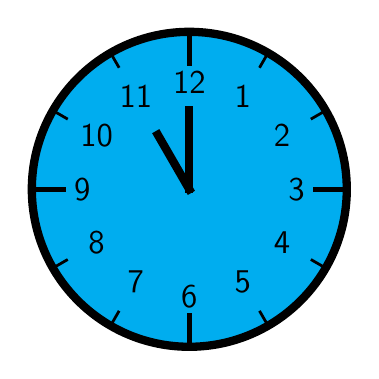
\begin{tikzpicture}[line cap=rect,line width=3pt]
\filldraw [fill=cyan] (0,0) circle [radius=2cm];
\foreach \angle [count=\xi] in {60,30,...,-270}
{
  \draw[line width=1pt] (\angle:1.8cm) -- (\angle:2cm);
  \node[font=\large] at (\angle:1.36cm) {\textsf{\xi}};
}
\foreach \angle in {0,90,180,270}
  \draw[line width=2pt] (\angle:1.6cm) -- (\angle:2cm);
\draw (0,0) -- (120:0.8cm);
\draw (0,0) -- (90:1cm);
\end{tikzpicture}
\end{center}
}

\section*{Atividades}

\num{1} Observe os horários nos relógios representados.

\begin{figure}[htpb!]
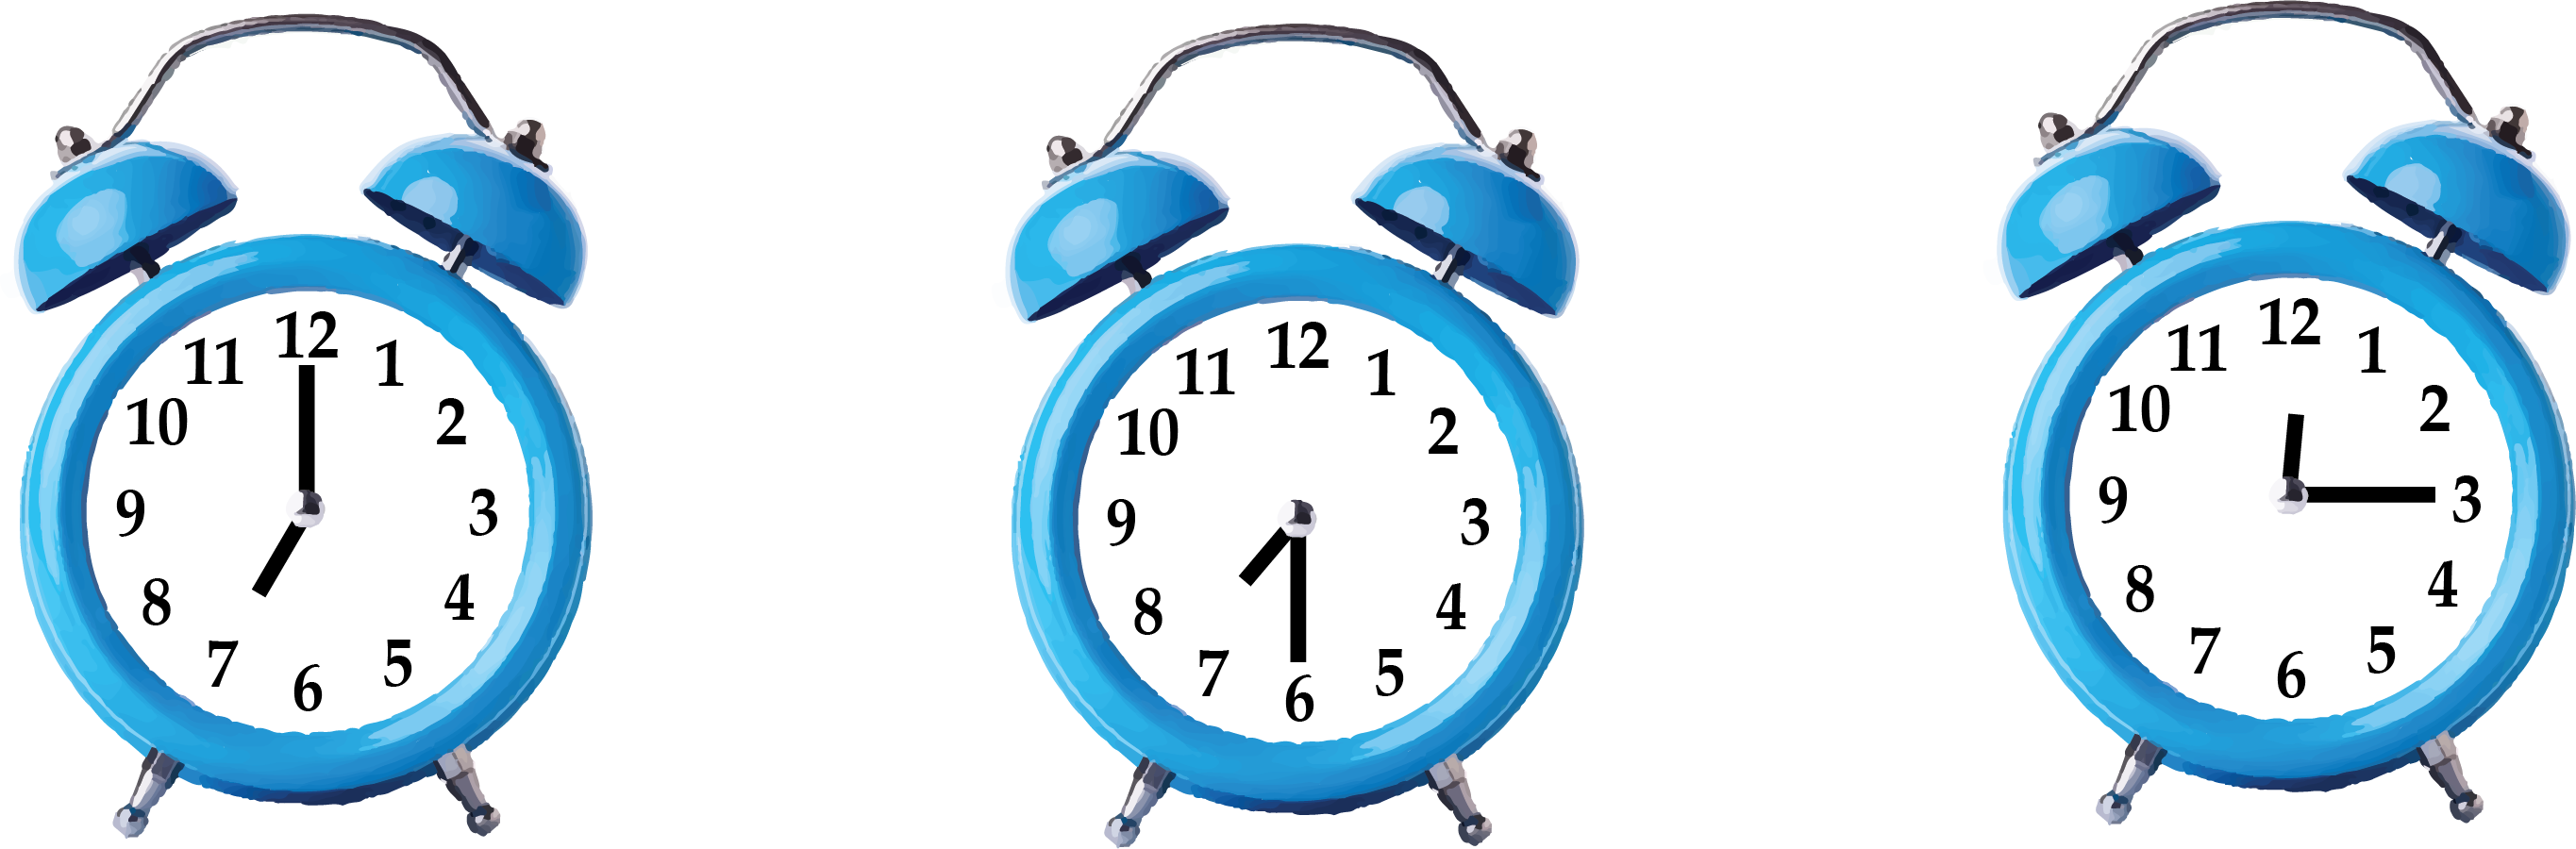
\includegraphics[width=\textwidth]{./media/image51.png}
\end{figure}

Qual o horário cada relógio está marcando?
\reduline{Estão representadas sete horas no primeiro relógio; sete e meia ou sete horas e trinta minutos no segundo relógio; e meio-dia e quinze minutos ou doze horas e quinze minutos no terceiro relógio.\hfill}
\linhas{2}

\pagebreak

\num{2} Observe o horário que os relógios digitais estão marcando:

\begin{figure}[htpb!]
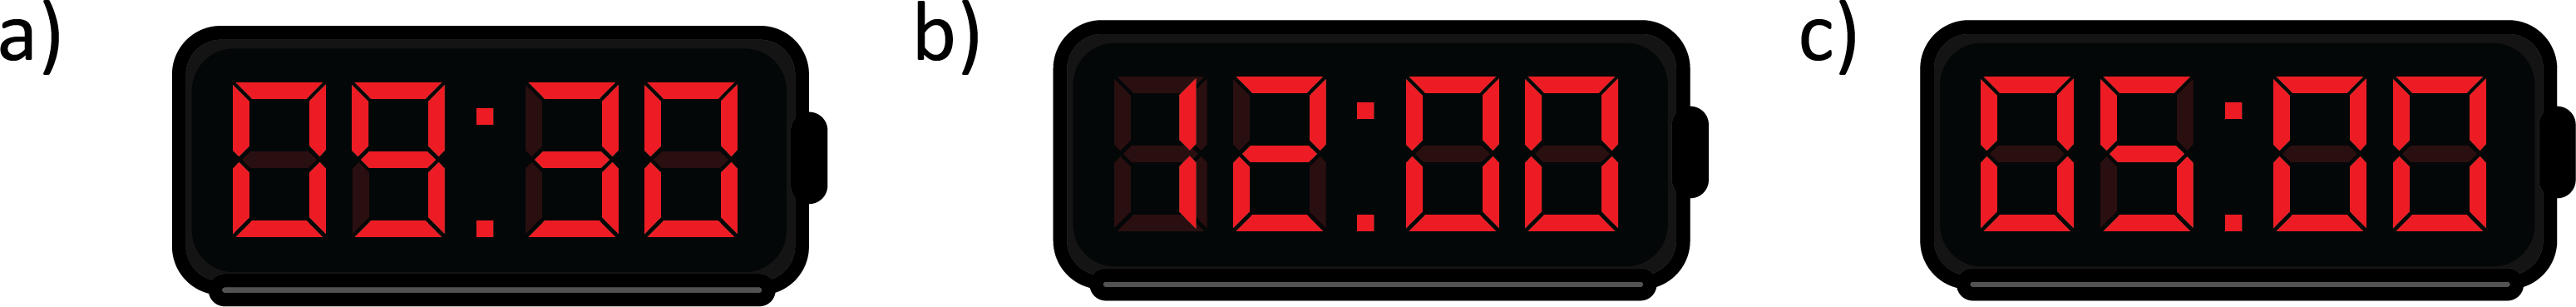
\includegraphics[width=\textwidth]{./media/image52.png}
\end{figure}

Como se lê cada um dos horários marcados?
\reduline{Estão representadas nove e meia ou nove horas e trinta minutos no primeiro relógio; meio-dia ou doze horas no primeiro relógio; e cinco horas no terceiro relógio.\hfill}
\linhas{1}

\num{3} A professora de Francisco colocou como primeira questão da prova a seguinte imagem:

\begin{figure}[htpb!]
\centering
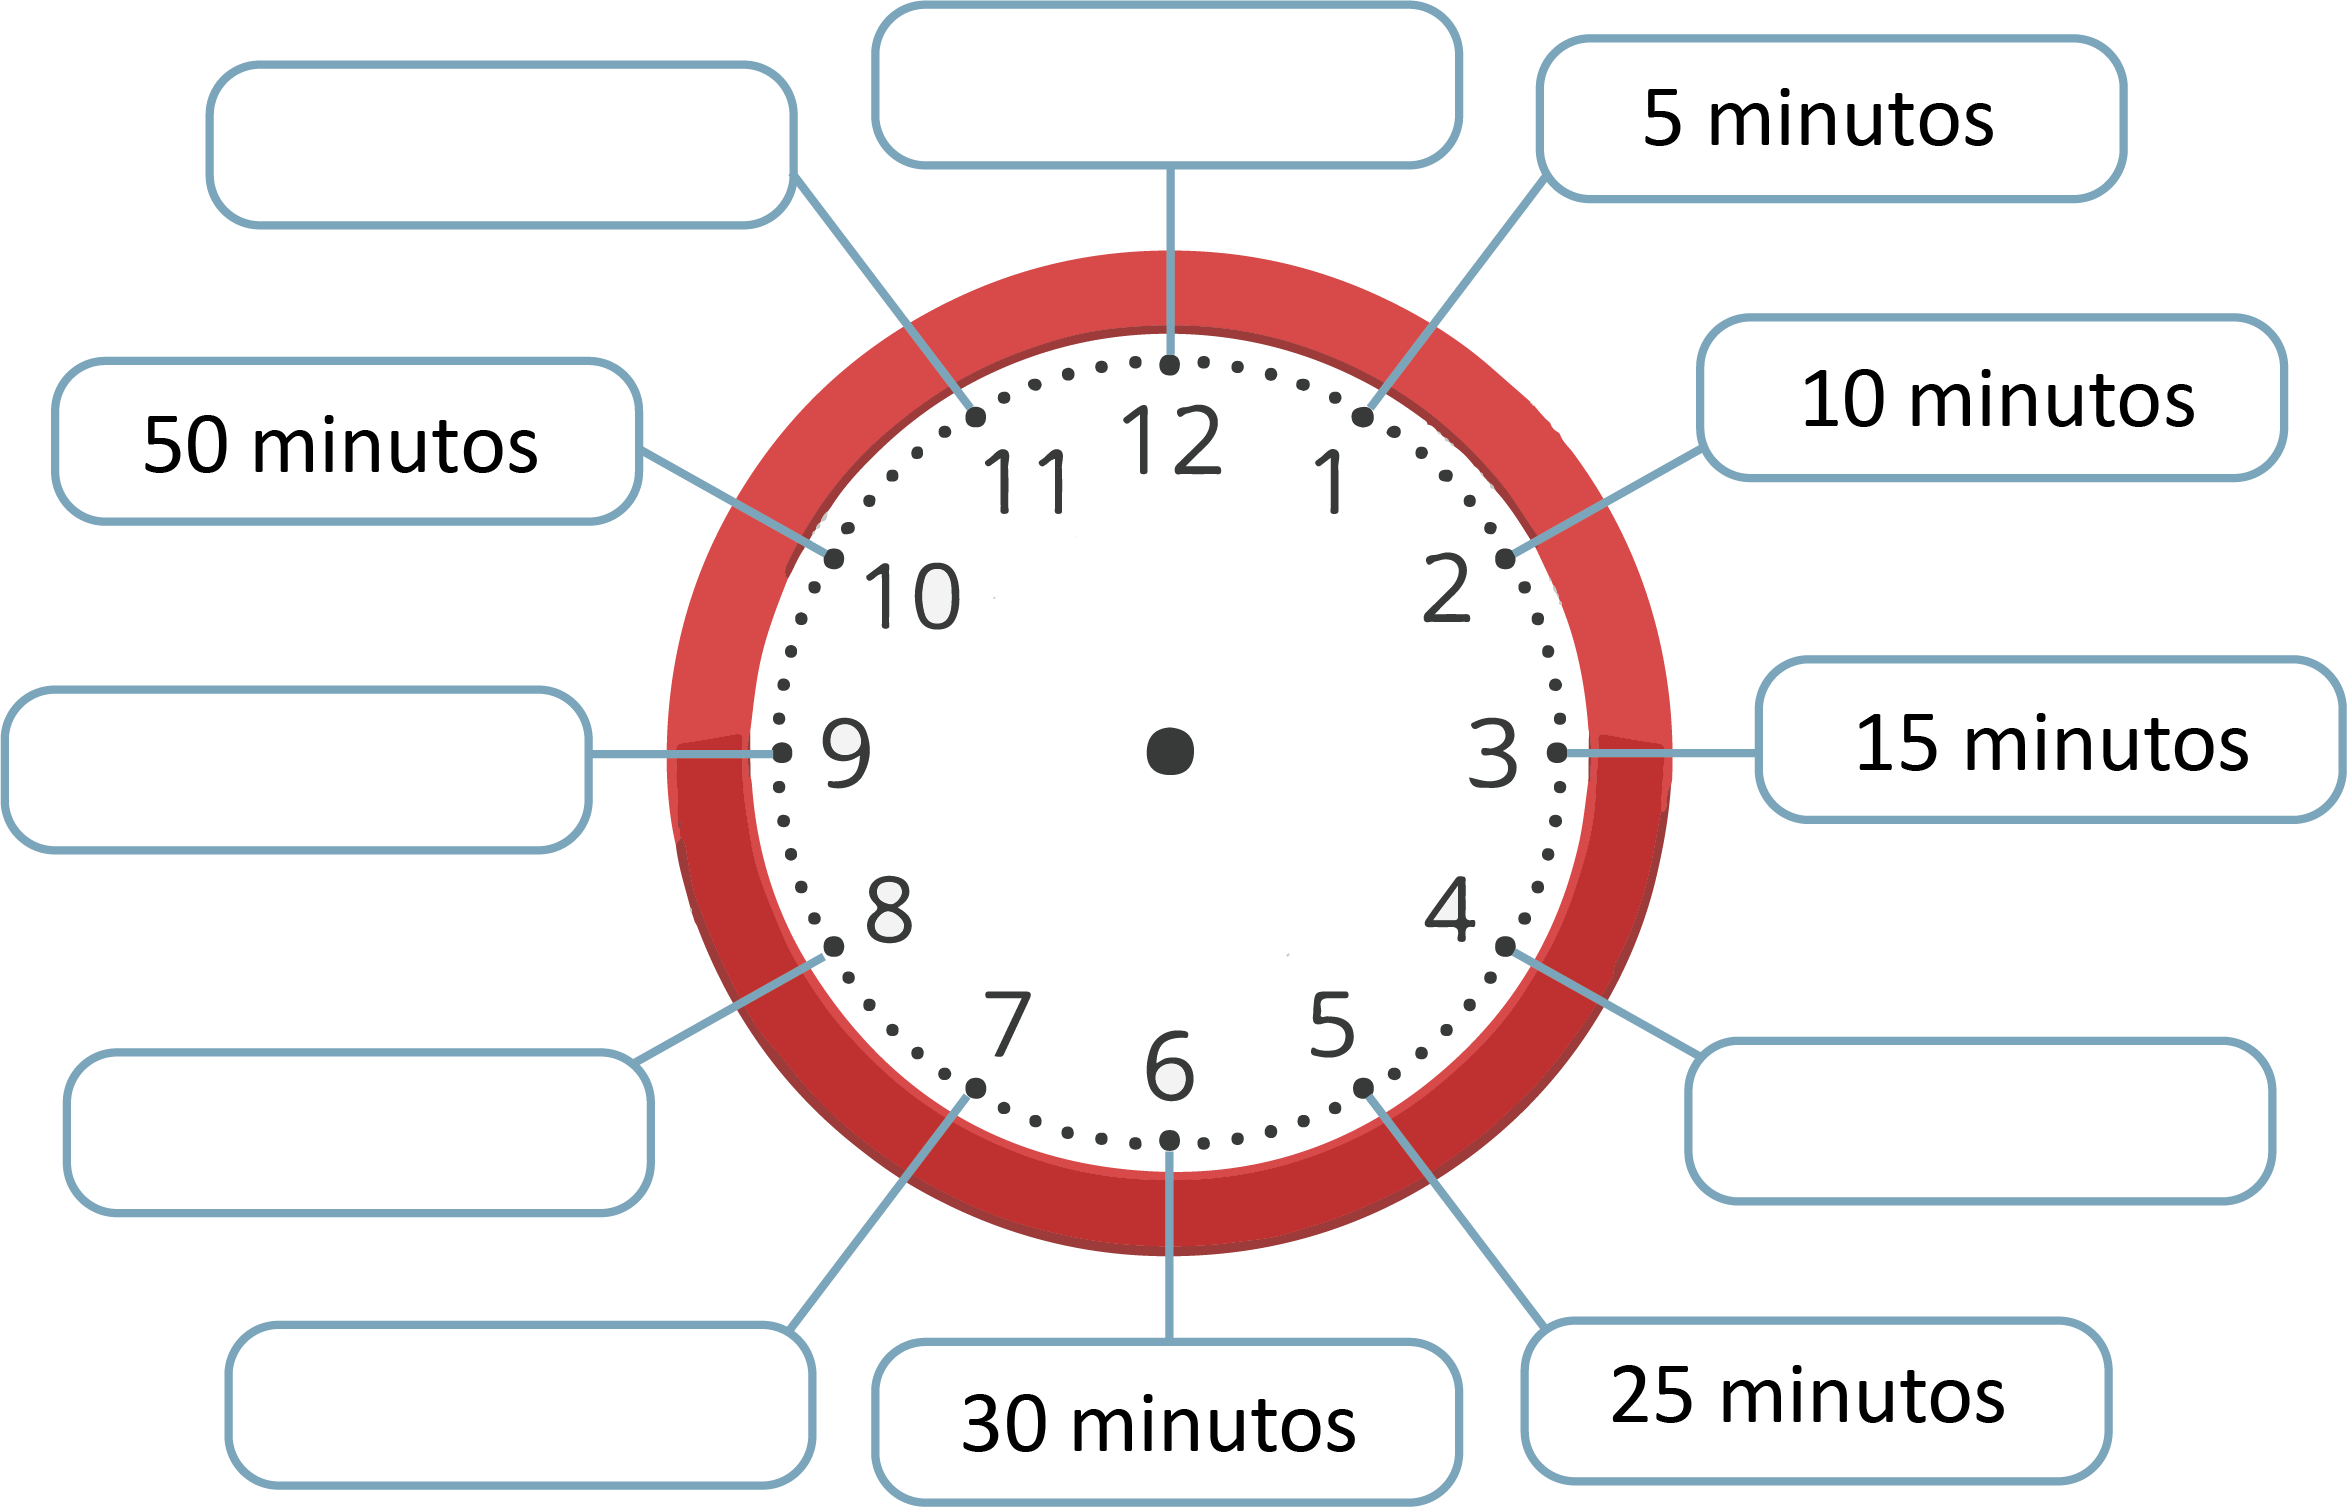
\includegraphics[width=\textwidth]{./media/image53.png}
\end{figure}

Ajude Francisco a completar os retângulos em branco com indicação de
minutos que cada um deles aponta.

\coment{20 minutos; 35 minutos; 40 minutos; 45 minutos; 55 minutos; 60 minutos.}

\pagebreak

\num{4} Observe o calendário e em seguida responda aos itens propostos.

\begin{figure}[htpb!]
\centering
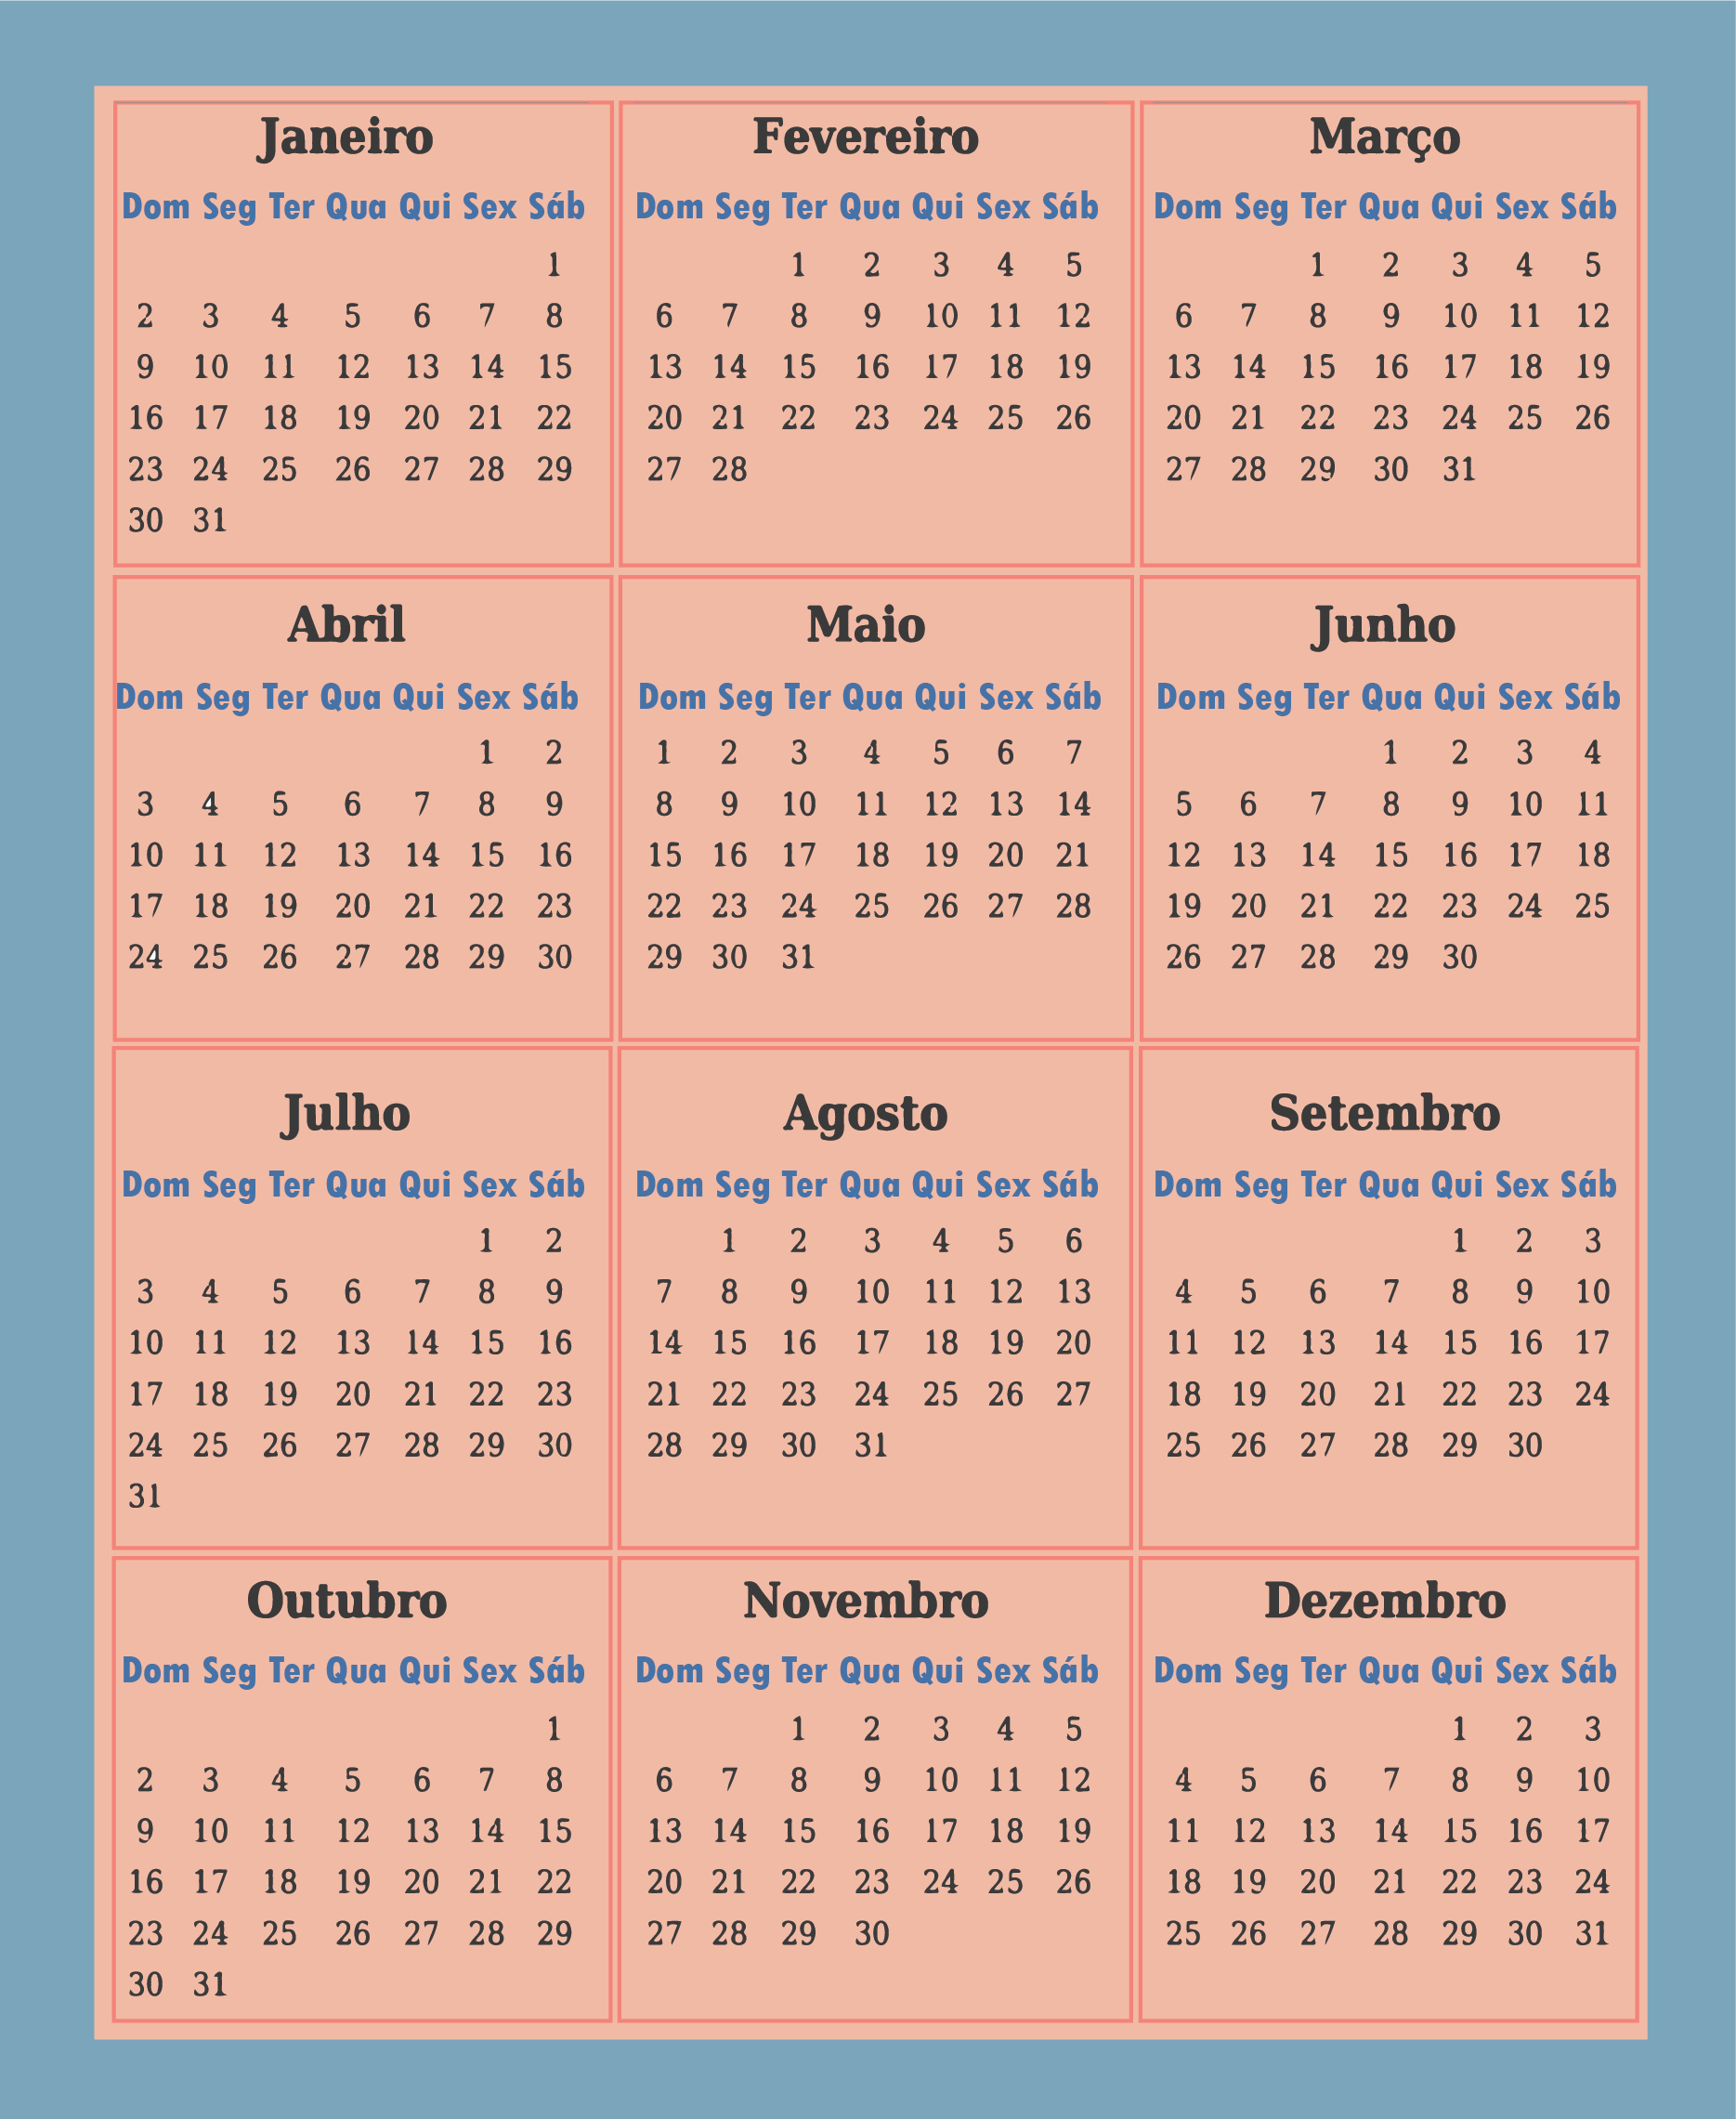
\includegraphics[width=\textwidth]{./media/image54.png}
\end{figure}

\pagebreak
\begin{escolha}
\item Circule no calendário o dia de seu aniversário.
%\reduline{Resposta pessoal.\hfill}

\item Agora, com um retângulo, marque o dia do aniversário de três colegas da sua sala.
%\reduline{Resposta pessoal.\hfill}

\item Marque com um triângulo o dia do aniversário de seu professor.
%\reduline{Resposta pessoal.\hfill}

\item Quantos anos você tem?
\reduline{Resposta pessoal.\hfill}

\item Você tem mais ou menos de 450 meses?
\reduline{Resposta pessoal.\hfill}
\end{escolha}

\num{5} O pai de Rafael estava conversando com um contador sobre o seu
faturamento semestral. Rafael escutou toda a conversa e depois fez os
seguintes questionamentos a seu pai:

O que é um semestre? 
Quantos semestres temos em um ano?

Diante de tantas perguntas, o pai de Rafael sentou-se com seu filho e
começou a responder aos questionamentos do filho.

Ajude o pai de Rafael a responder corretamente a todas as perguntas que o filho lhe fez.
\reduline{Um semestre é um período composto por 6 meses e em um ano temos 2 semestres.\hfill}

\num{6} Marque, desenhando no relógio analógico abaixo, os ponteiros das horas e o dos
minutos na posição exata em que estarão para representar o horário em que
suas aulas começam.

\begin{figure}[htpb!]
\centering
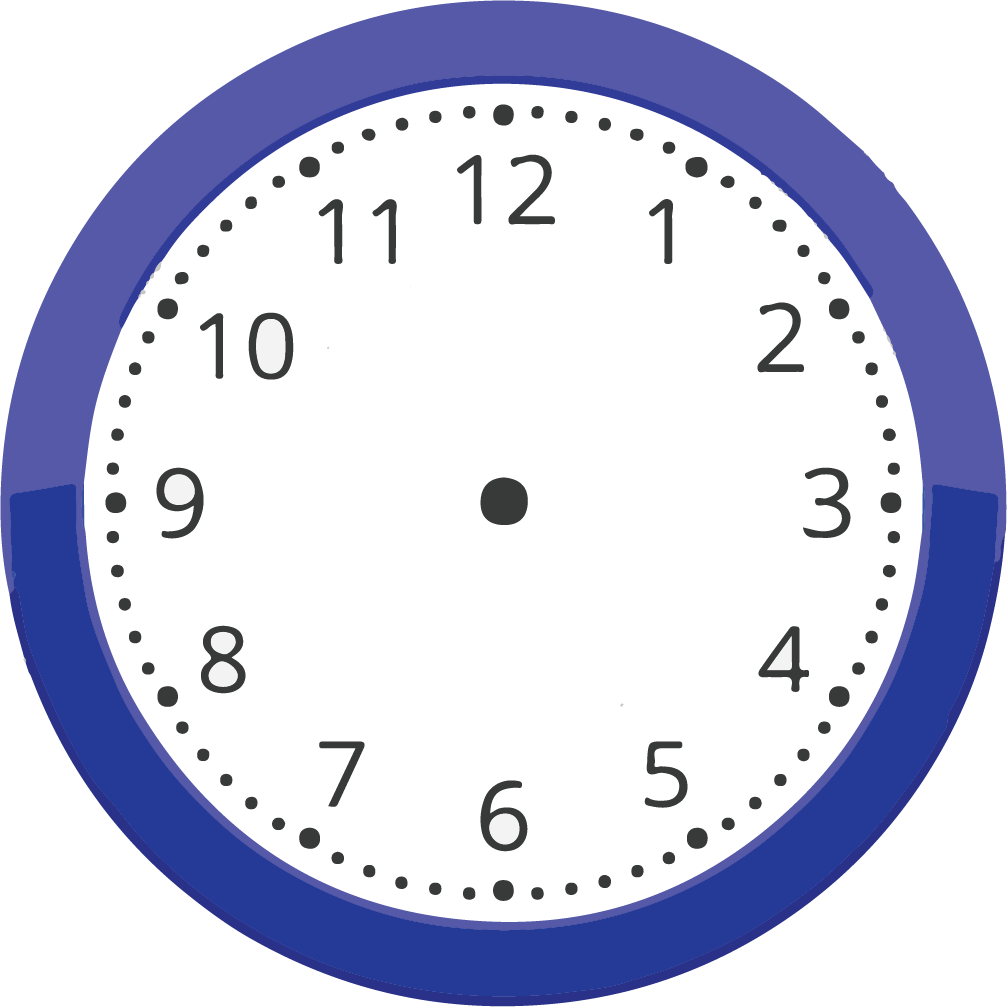
\includegraphics[width=0.3\textwidth]{./media/image54b.png}
\end{figure}

\coment{Resposta circunstancial. Dependerá do horário de início das aulas.}

\pagebreak

\num{7} Aos finais de semana, Renato anda de bicicleta ao redor da praça do bairro onde mora.

\begin{figure}[htpb!]
\centering
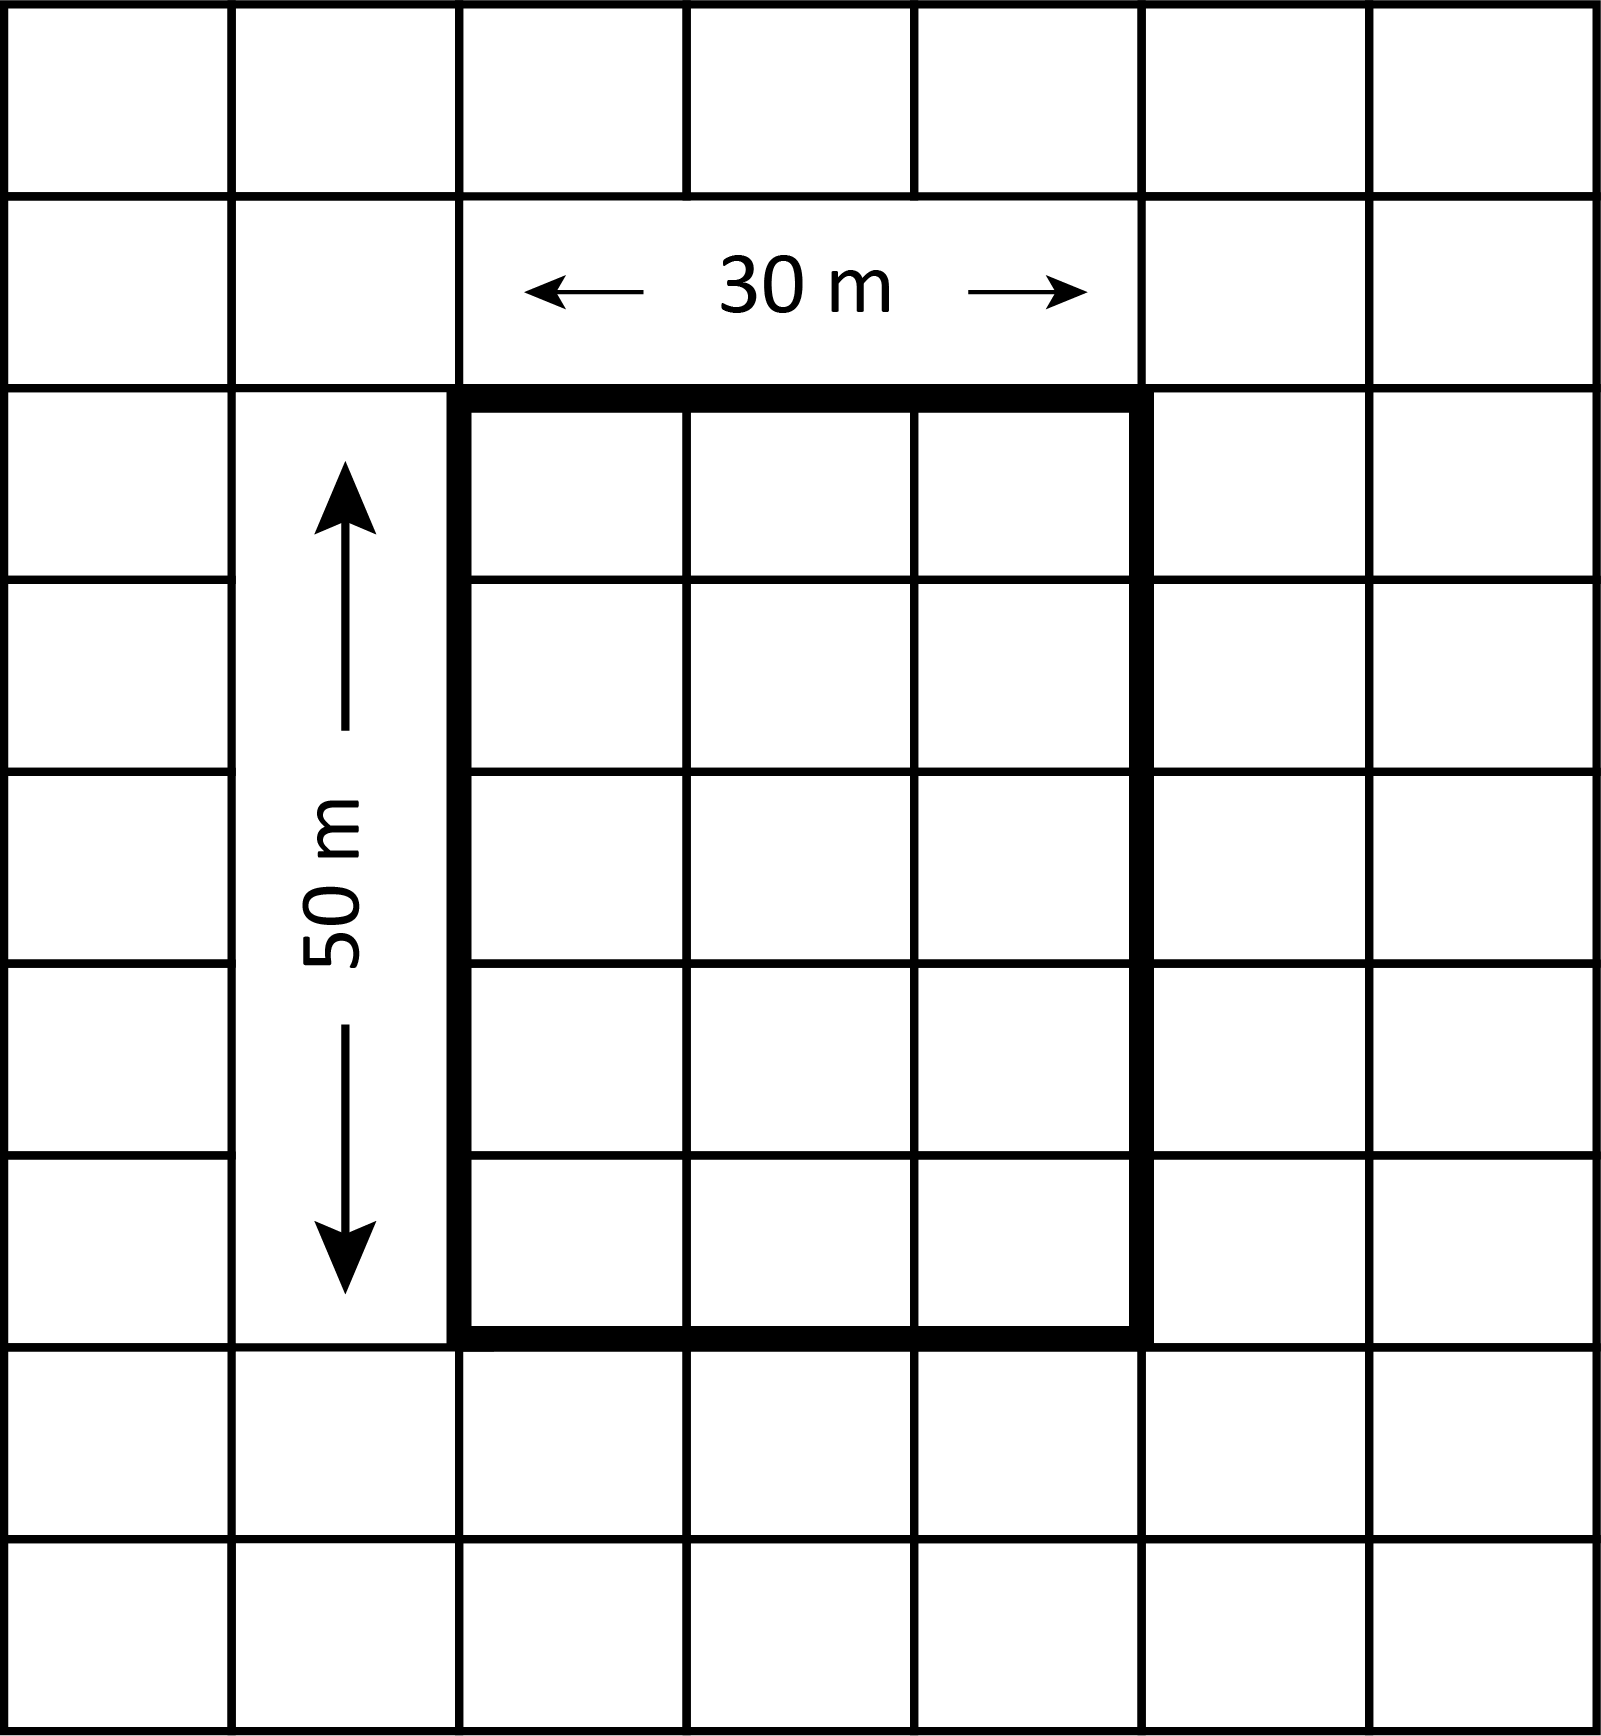
\includegraphics[width=.4\textwidth]{./media/image55.png}
\end{figure}

Se ele der duas voltas completas ao redor da praça, qual é a distância que ele percorrerá?

\reduline{(2 x 30 + 2 x 50) x 2 = 320 m. Sempre que possível, estimule a montagem da expressões, para que os alunos comecem a se acostumar.\hfill}
\linhas{1}

\num{8} As figuras a seguir foram desenhadas em uma malha quadriculada.

\begin{figure}[htpb!]
\centering
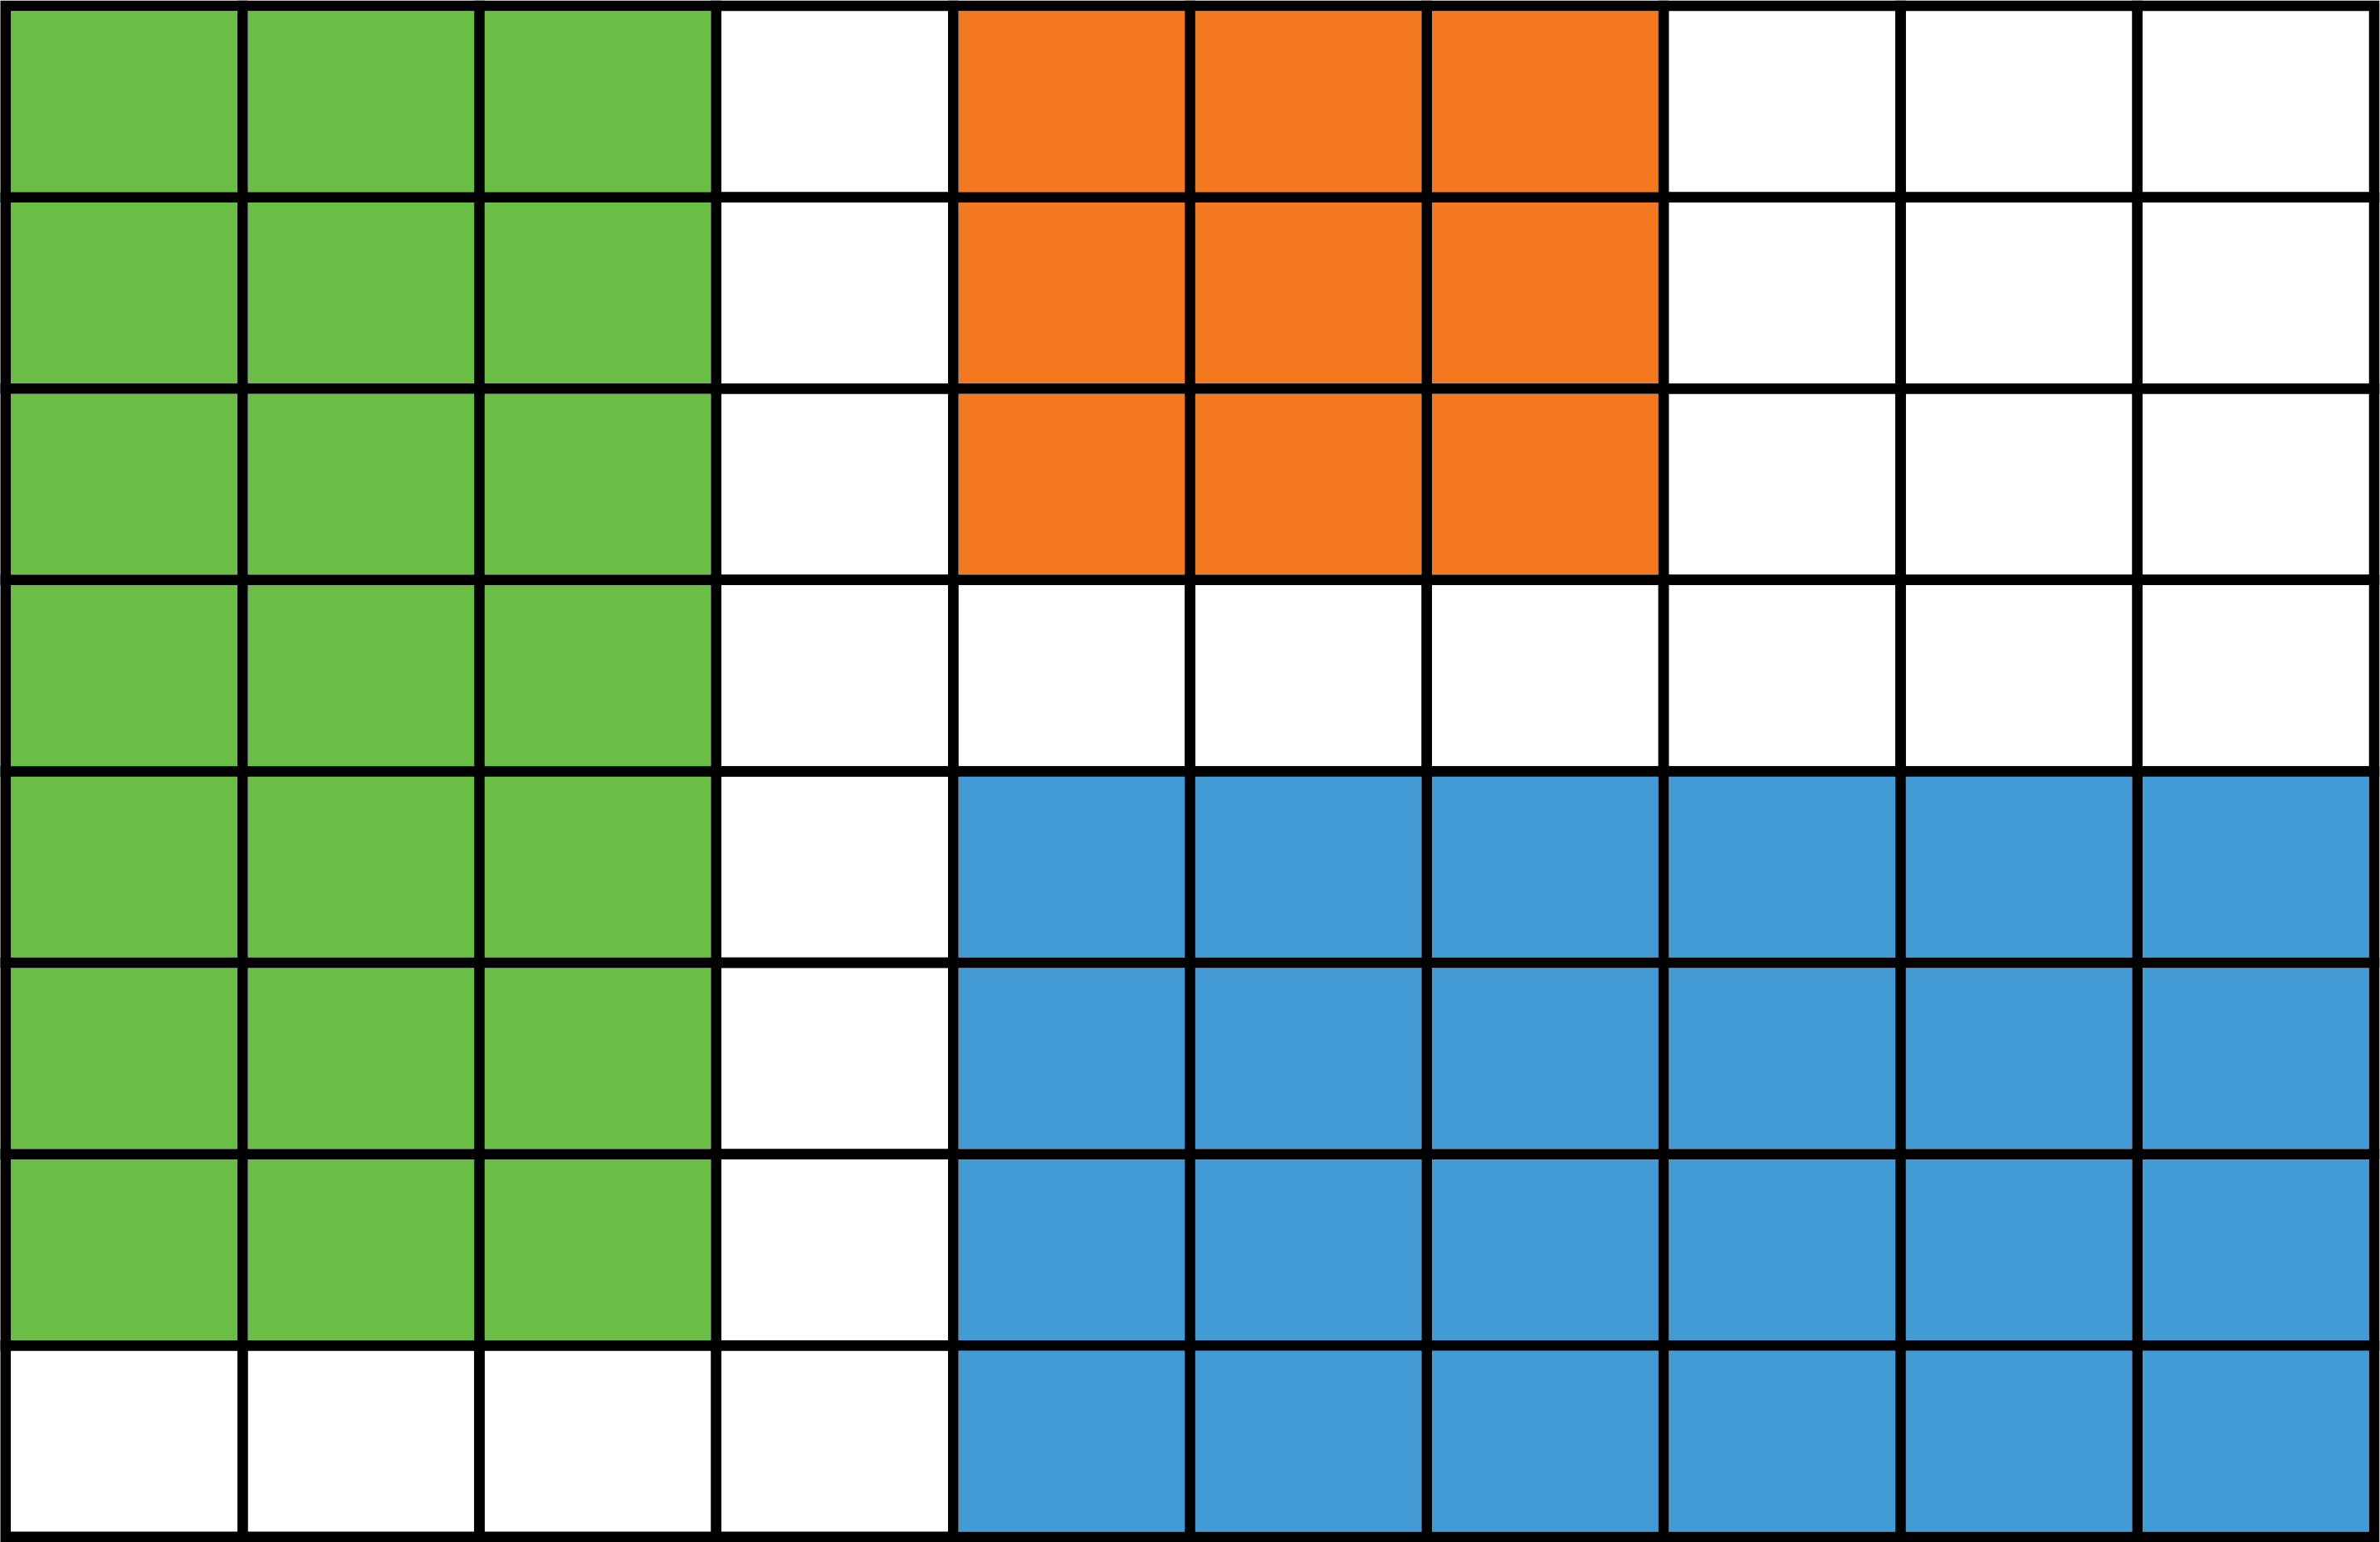
\includegraphics[width=0.5\textwidth]{./media/image56.png}
\end{figure}

Quantos quadradinhos pintados cada figura possui?
\reduline{Verde: 21 quadradinhos; azul: 24 quadradinhos; e laranja: 9 quadradinhos.\hfill}
\linhas{1}

\num{9} Na malha quadriculada, cada quadrado representa uma área de 10 metros quadrados.

\begin{figure}[htpb!]
\centering
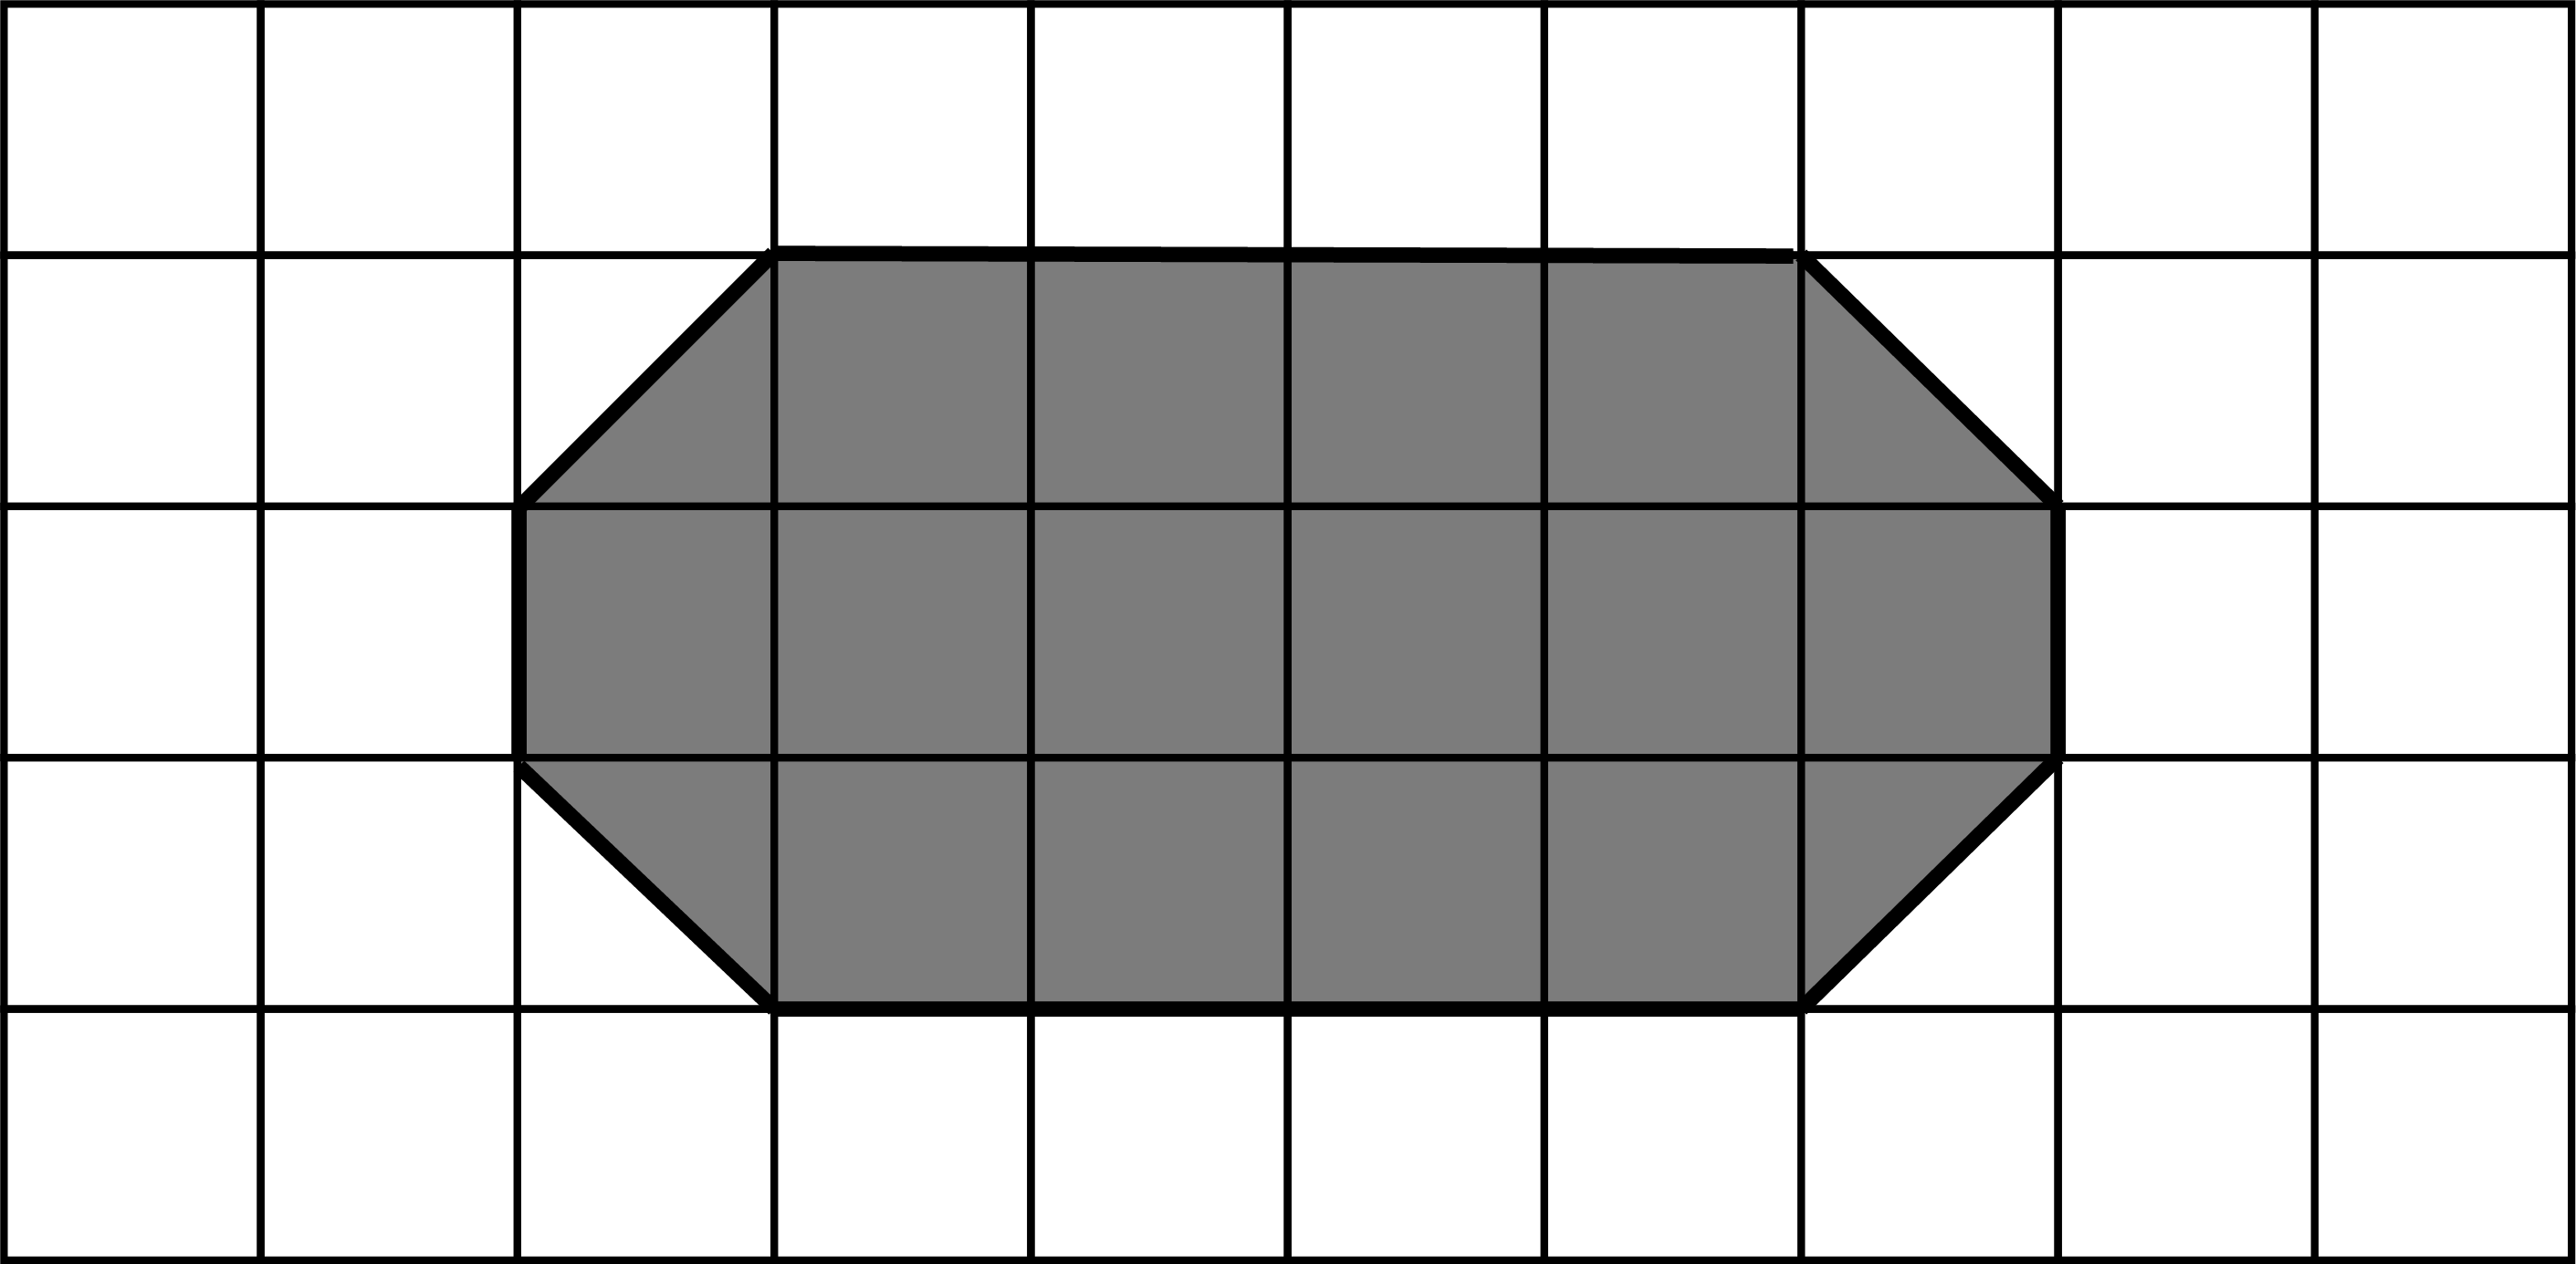
\includegraphics[width=.6\textwidth]{./media/image60.png}
\end{figure}

Qual é a área que a figura ocupa na malha quadriculada?
\reduline{Realizando a contagem de quadradinhos que preenchem a figura, chega-se à conclusão de que, para o preenchimento dela, são necessários 16 quadradinhos. Portanto, 16 x 10 = 160 metros quadrados.\hfill}

\vspace{2em}

\num{10} Utilizando sua régua, una pontos e faça uma figura na malha, representada apenas pelos pontinhos. Em seguida, mostre sua
figura para um colega e veja se ele descobre o que você representou.

\begin{figure}[htpb!]
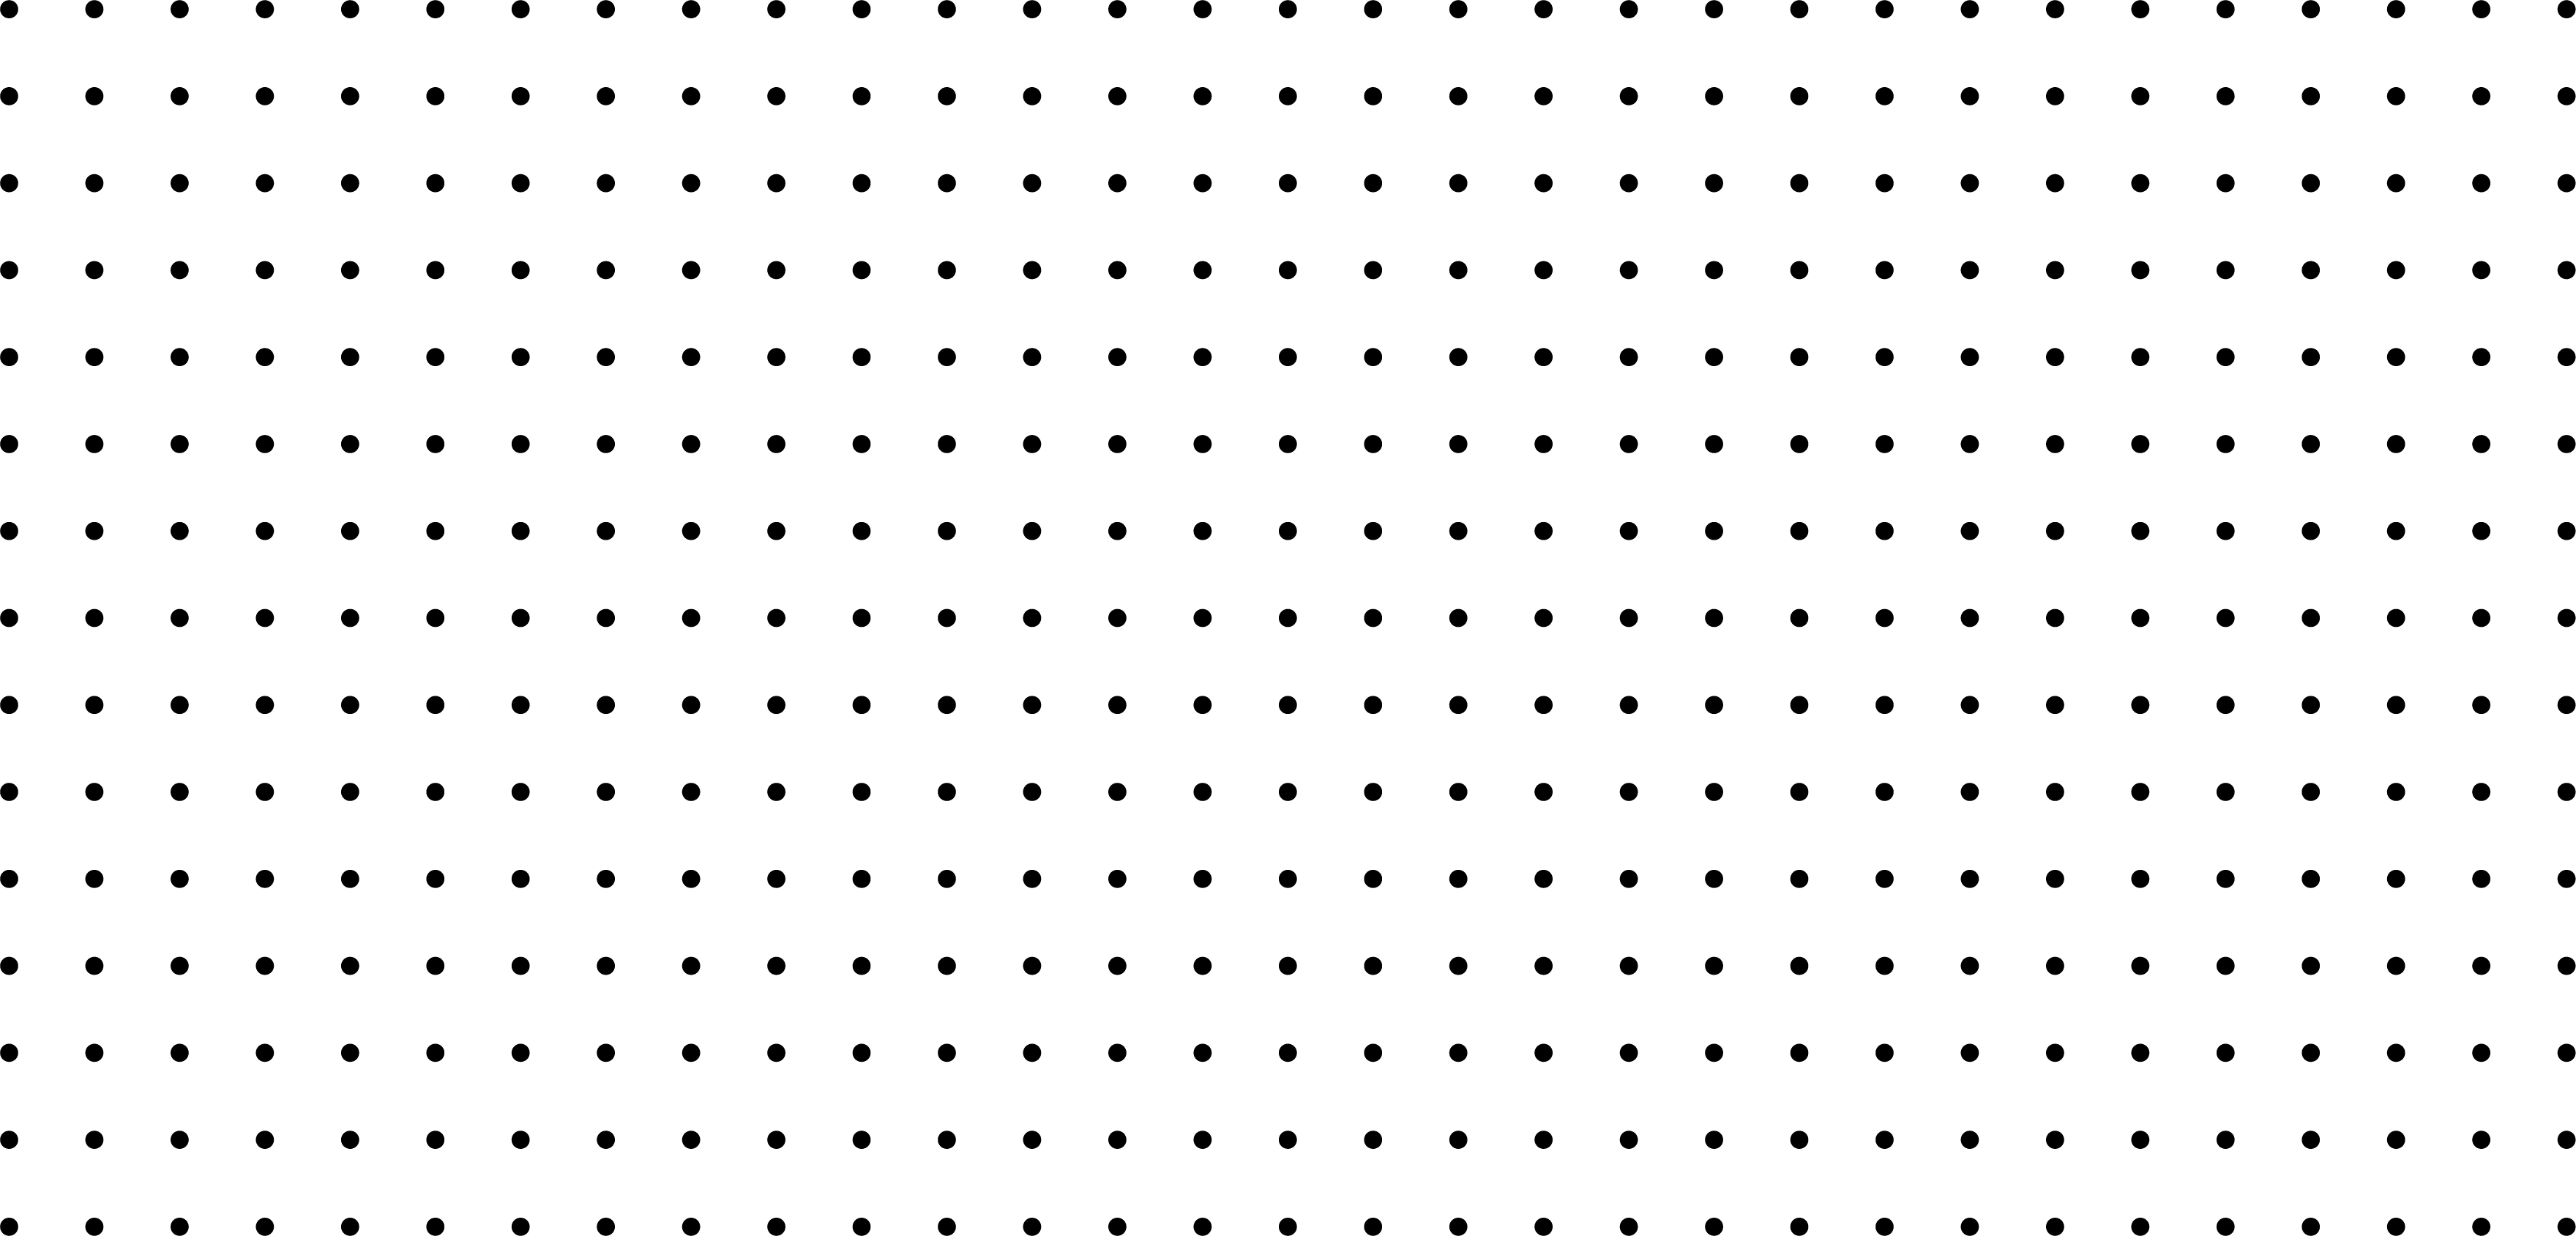
\includegraphics[width=\textwidth]{./media/image58.png}
\end{figure}

\coment{Resposta pessoal.}

\num{11} Os desenhos representados foram feitos com o auxílio de uma malha
quadriculada na qual cada lado de quadradinho mede 1 cm.

\begin{figure}[htpb!]
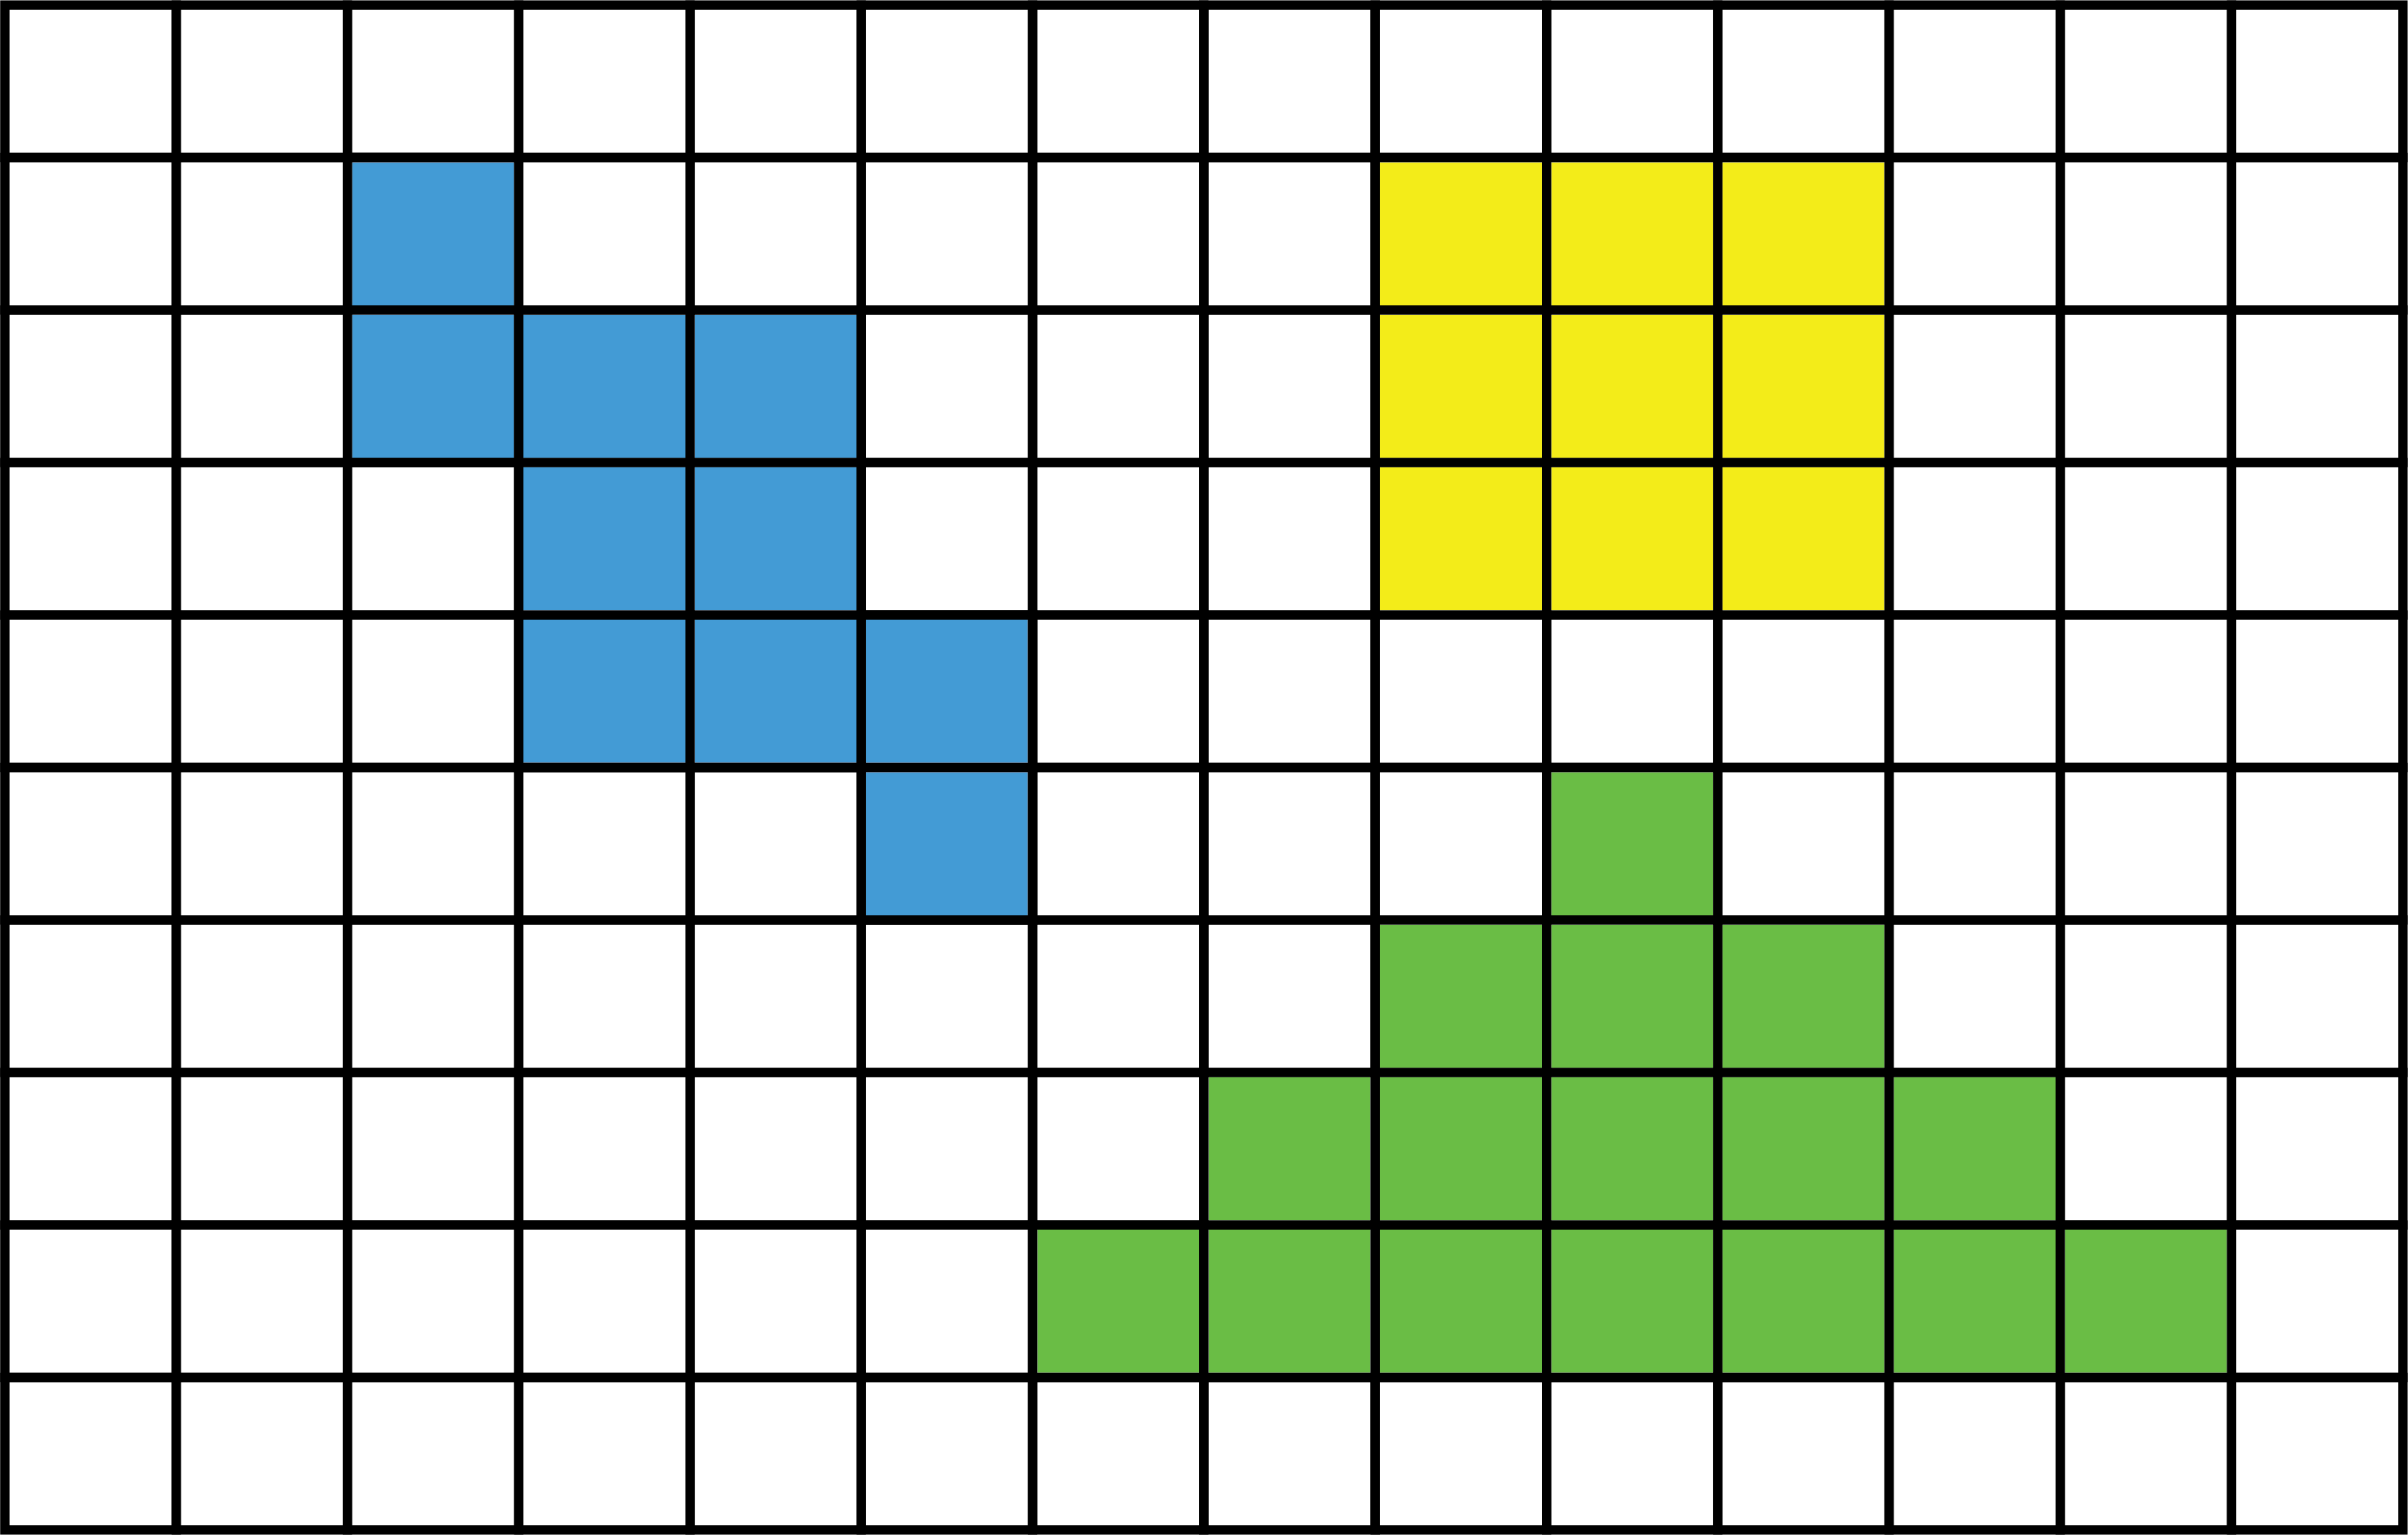
\includegraphics[width=\textwidth]{./media/image57.png}
\end{figure}

\begin{escolha}
\item Qual a medida, em centímetros, do contorno da figura azul?
\reduline{18 cm\hfill}
\linhas{1}

\item Qual a medida, em centímetros, do contorno da figura amarela?
\reduline{12 cm\hfill}
\linhas{1}

\item Qual a medida, em centímetros, do contorno da figura verde?
\reduline{22 cm\hfill}
\linhas{1}
\end{escolha}


\begin{comment}
\num{11} Observe atentamente as figuras.

\begin{figure}[htpb!]
\centering
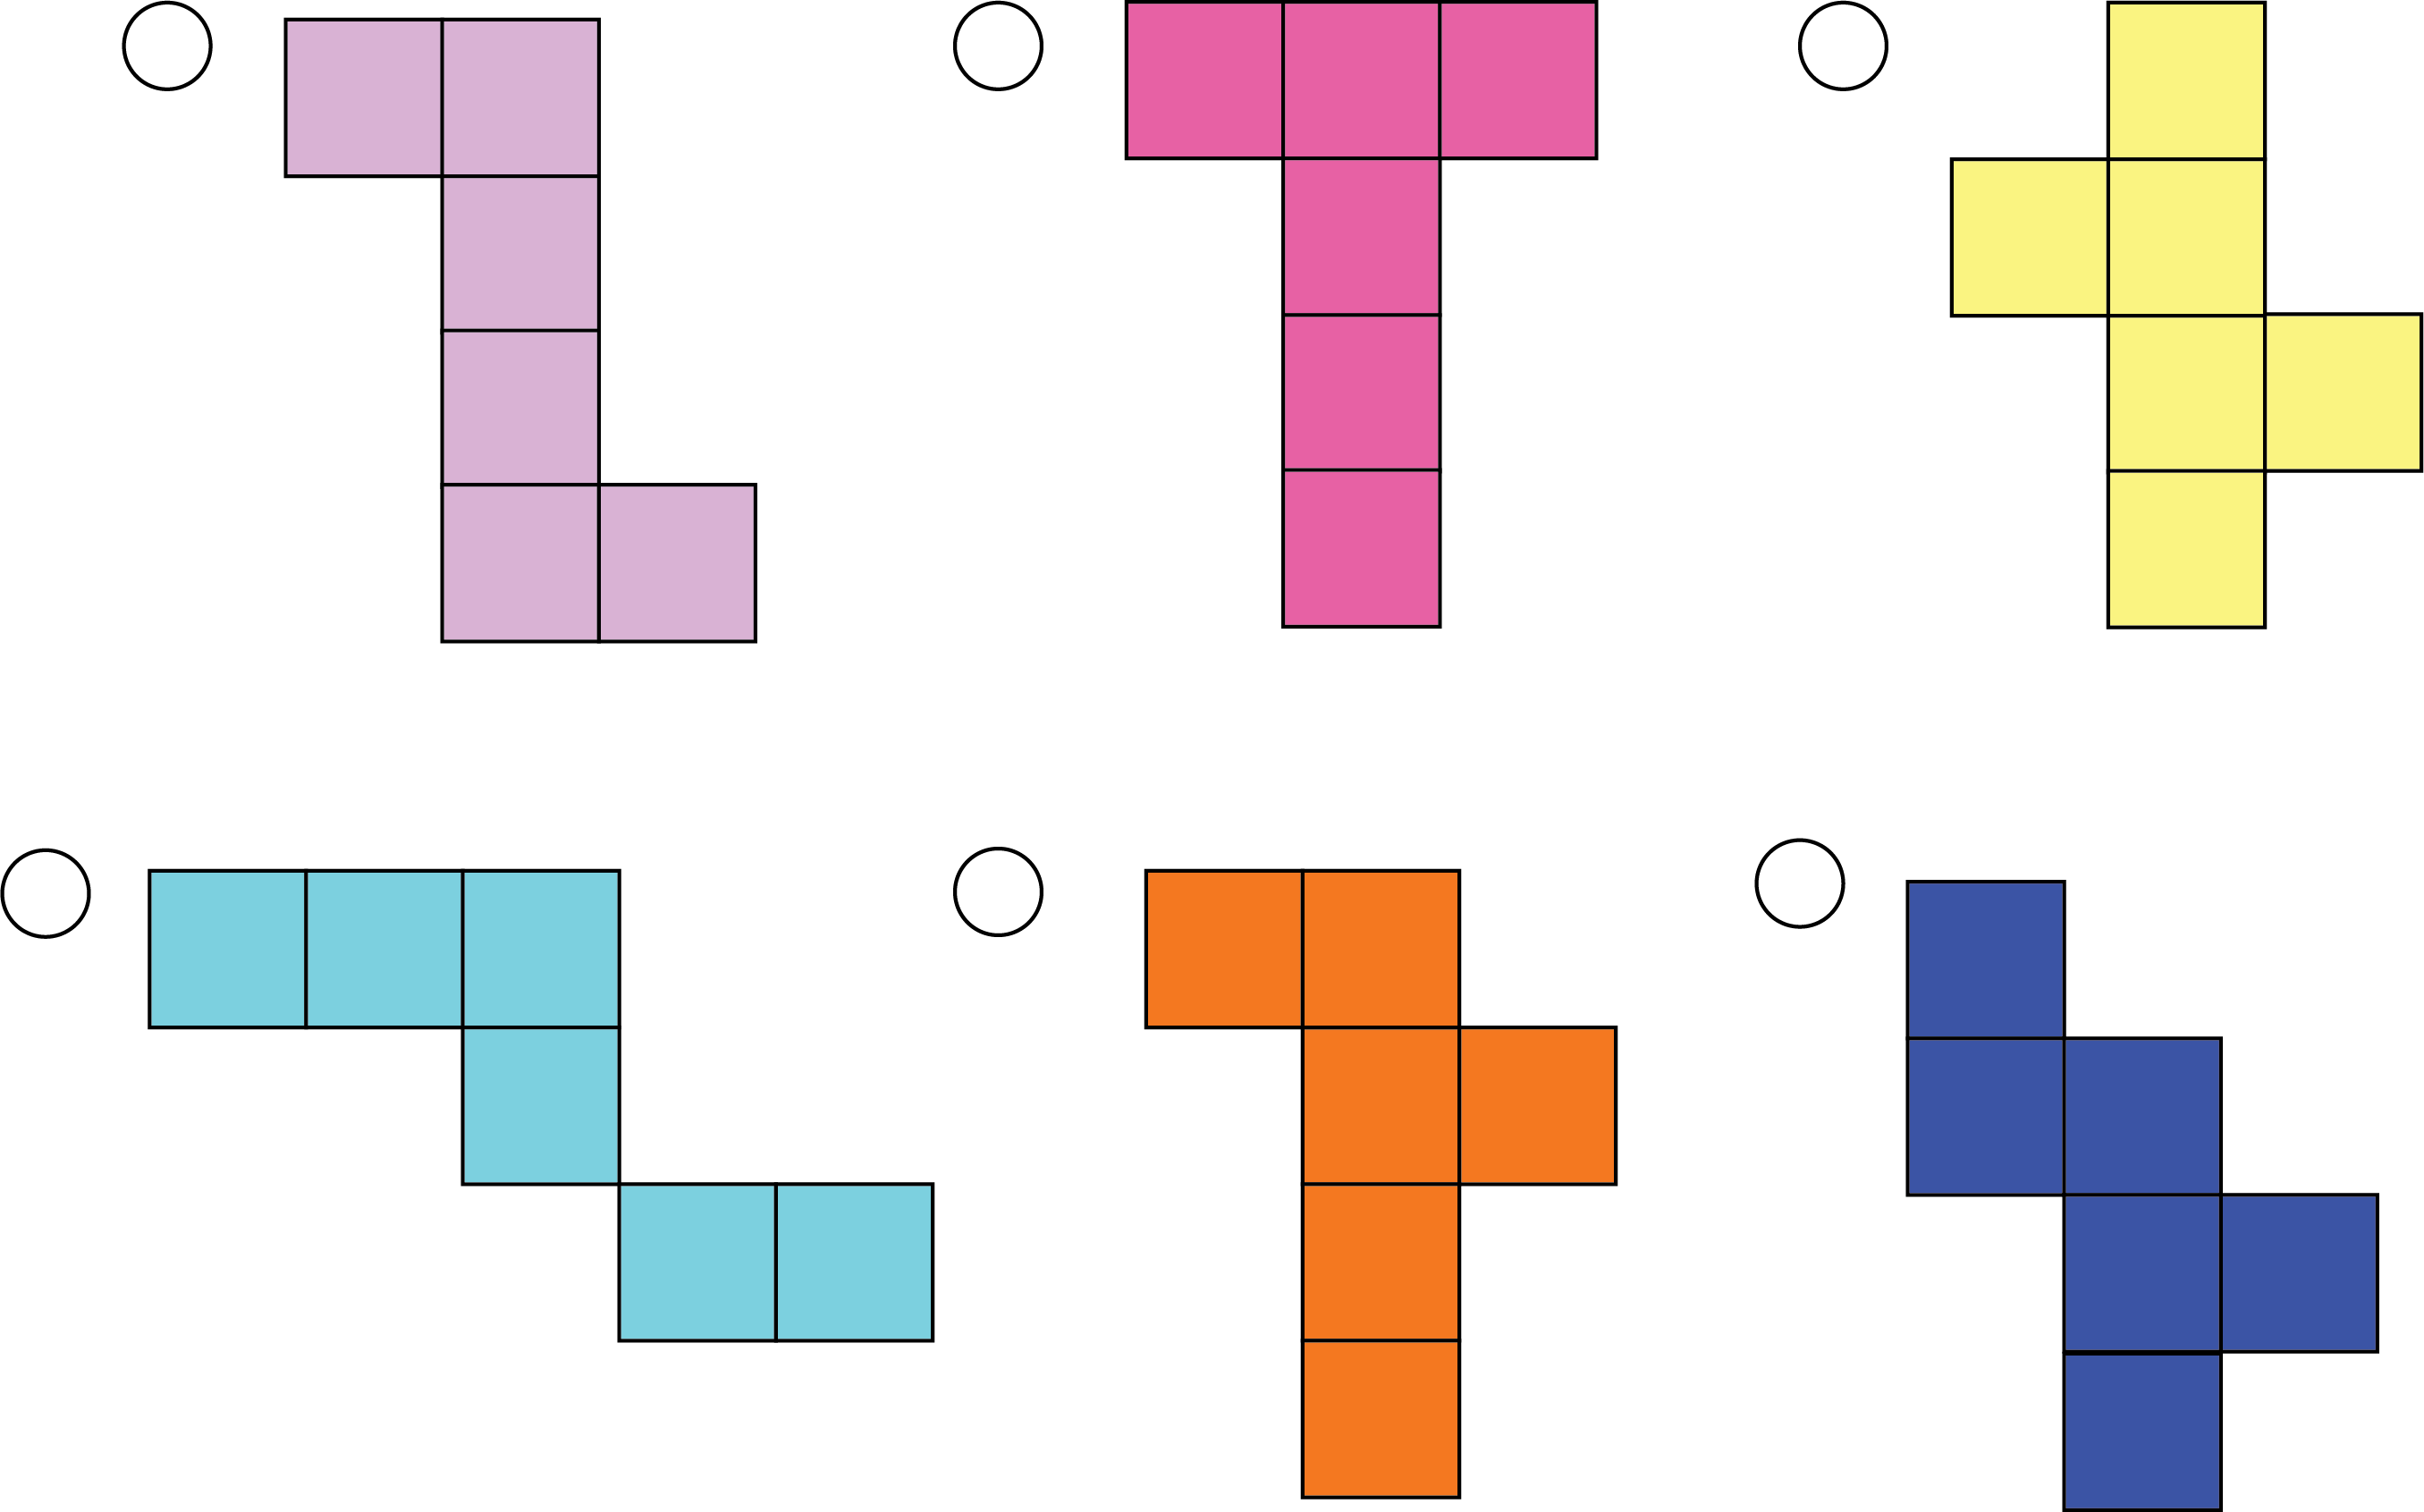
\includegraphics[width=.6\textwidth]{./media/image59.png}
\end{figure}

Quais delas possuem a mesma quantidade de quadradinhos? Justifique sua resposta.
\reduline{Todas são compostas pelo mesmo número de quadradinhos.\hfill}
\linhas{2}
\end{comment}

\section*{Treino}

\num{1} Paulo resolveu ir a uma exposição e, no momento, encontra-se na
bilheteria. Quanto ele precisará andar para chegar à exposição,
considerando o caminho destacado, sabendo-se que o lado de cada
quadradinho da malha tem medida de 3m?

\begin{figure}[htpb!]
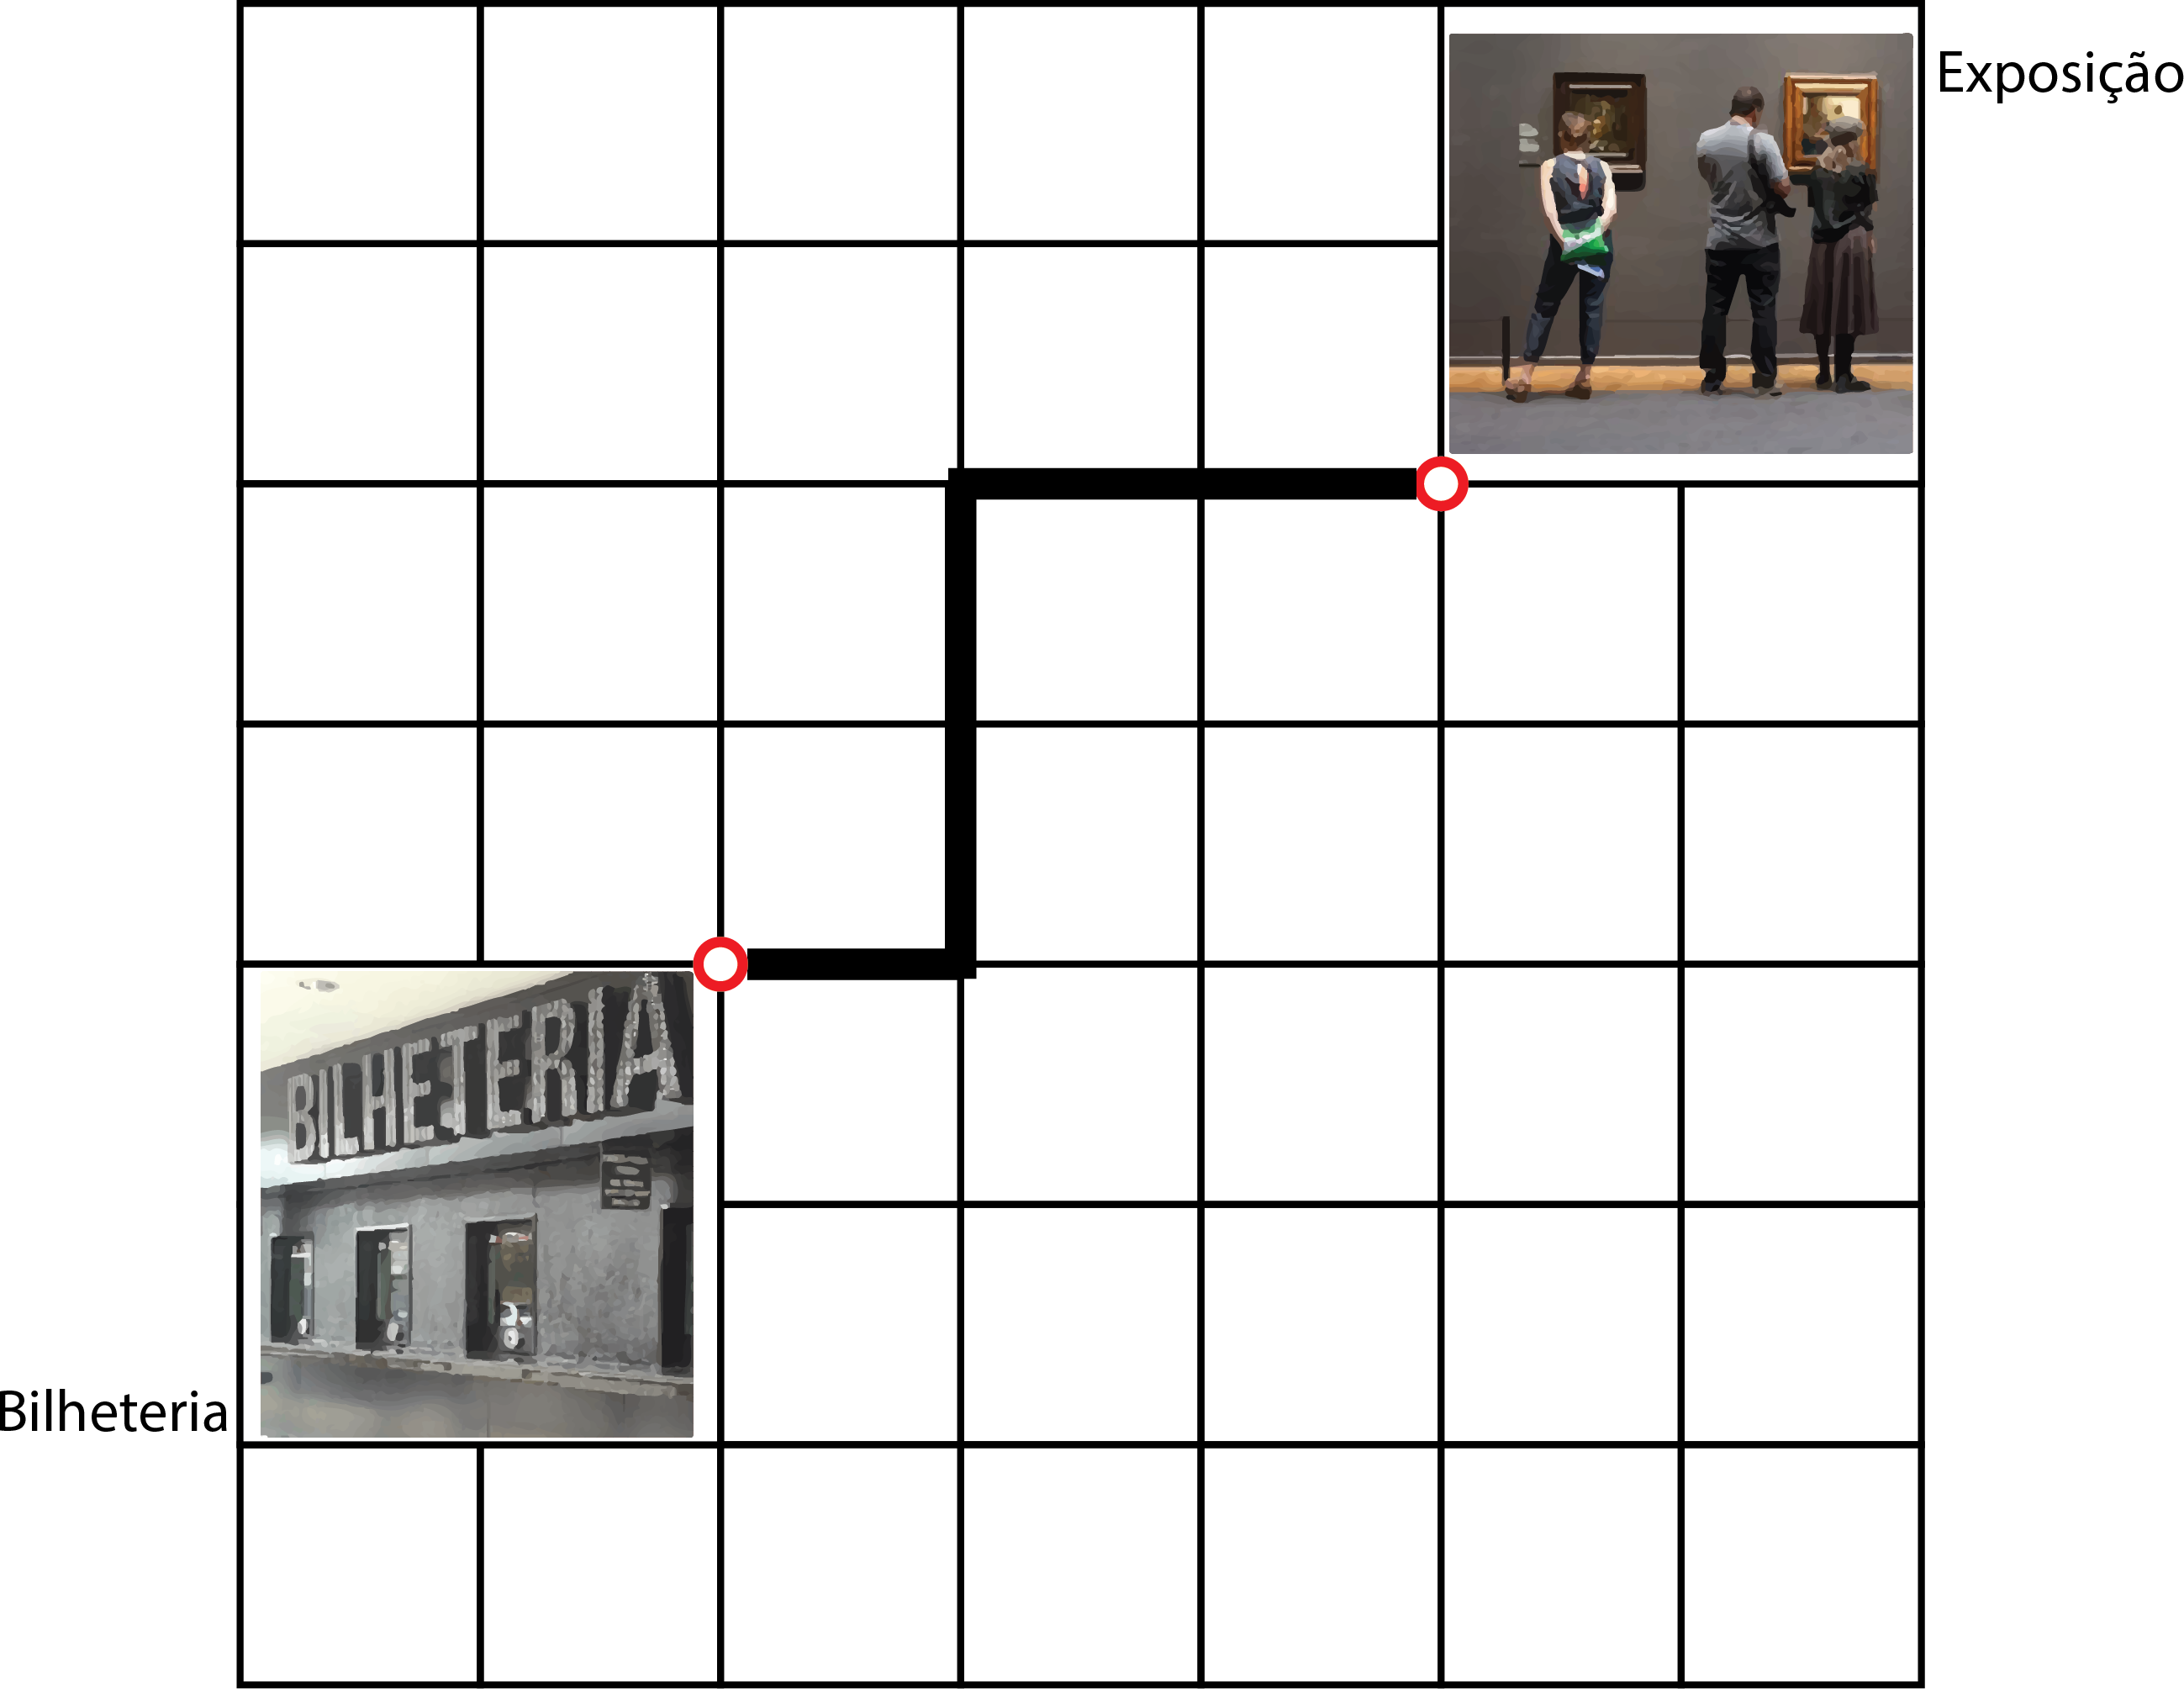
\includegraphics[width=\textwidth]{./media/image61.png}
\end{figure}

\begin{escolha}
\item
  5 m.
\item
  10 m.
\item
  12 m.
\item
  15 m.
\end{escolha}

\pagebreak

\num{2} Amanda quer fazer seu nome em letras bem grandes em um papel colorido para enfeitar sua festa de aniversário. Para as letras terem tamanhos equivalentes, resolveu, primeiro, desenhá-las em um papel quadriculado. Veja o A que ela fez.

Quantos quadrados, de forma aproximada, esse A ocupa?

\begin{figure}[htpb!]
\centering
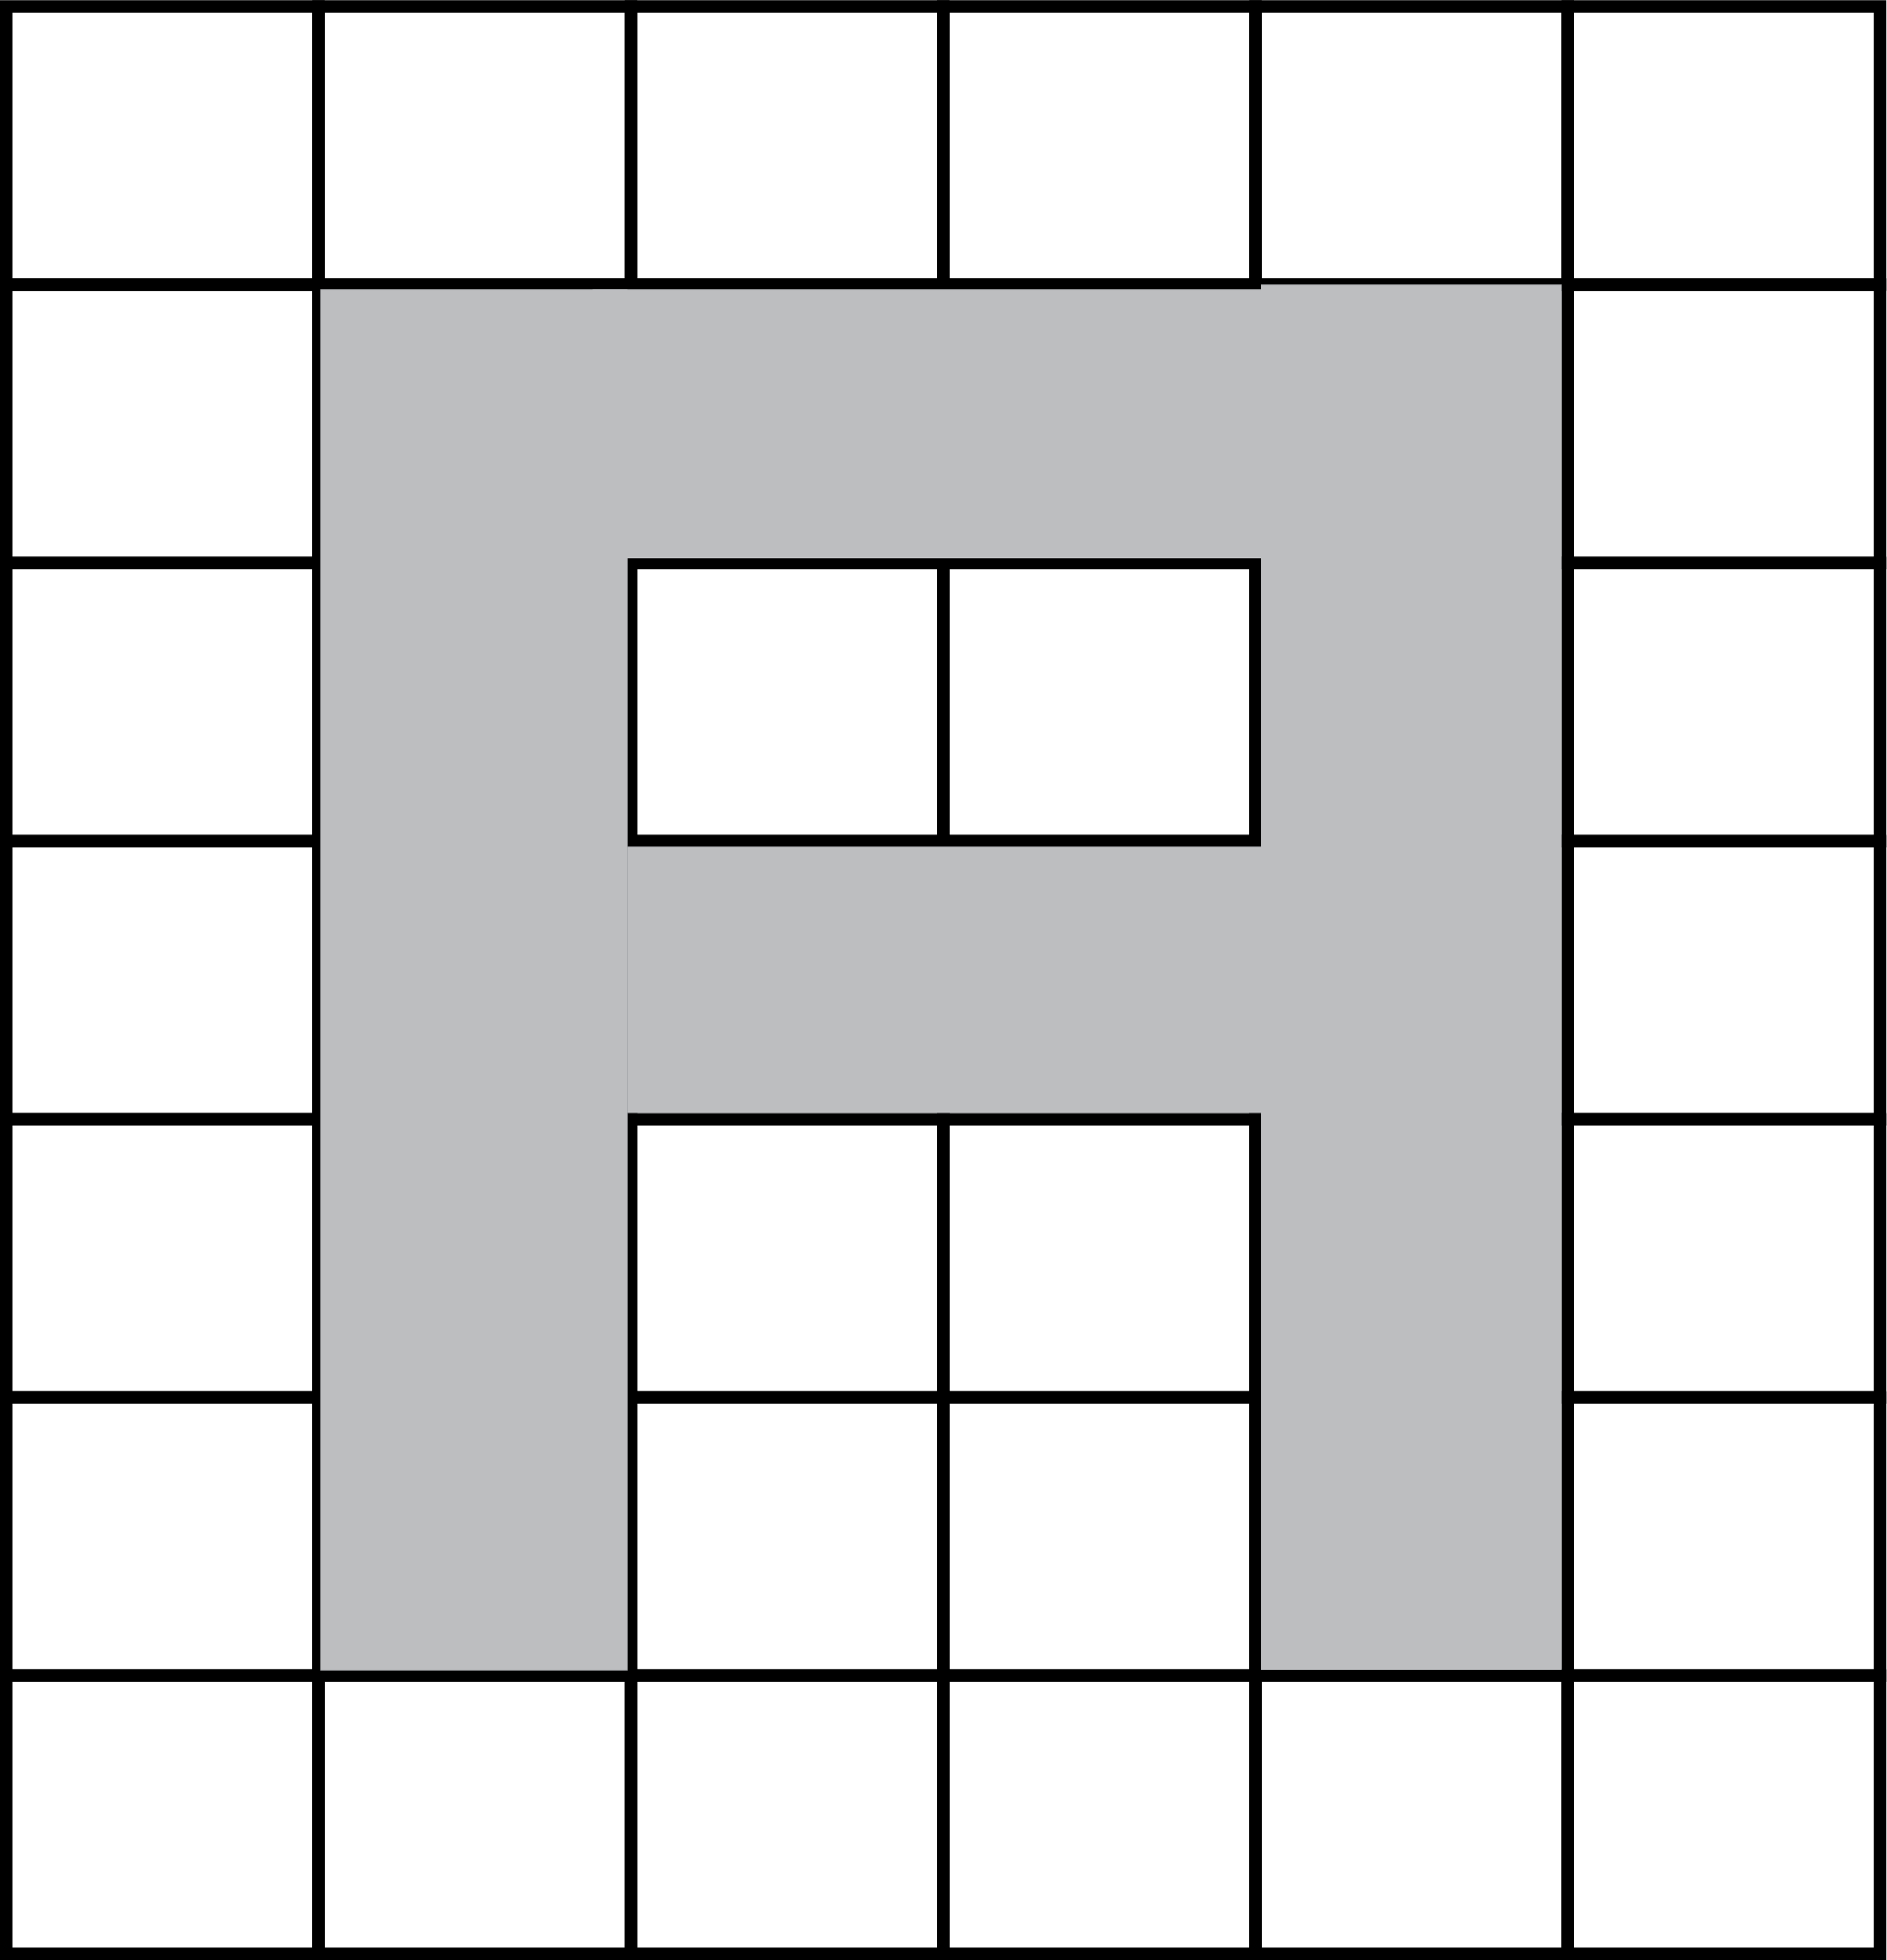
\includegraphics[width=.8\textwidth]{./media/image62.png}
\end{figure}

\begin{escolha}
\item
  3.
\item
  9.
\item
  26.
\item
  120.
\end{escolha}

\pagebreak
\num{3} Leia a notícia.

\begin{quote}
A cidade de Tombalina ganhará uma nova praça. A praça atual, com a famosa pista de corrida de 25 metros, será substituída por outra, com pista de corrida e caminhada de 125 metros de comprimento.

A nova praça será construída no centro da cidade, em uma área verde que atualmente não está sendo utilizada. A prefeitura investirá na criação de um espaço amplo e agradável para a população, com áreas de lazer e convivência.

\vspace{1em}
\begin{center}
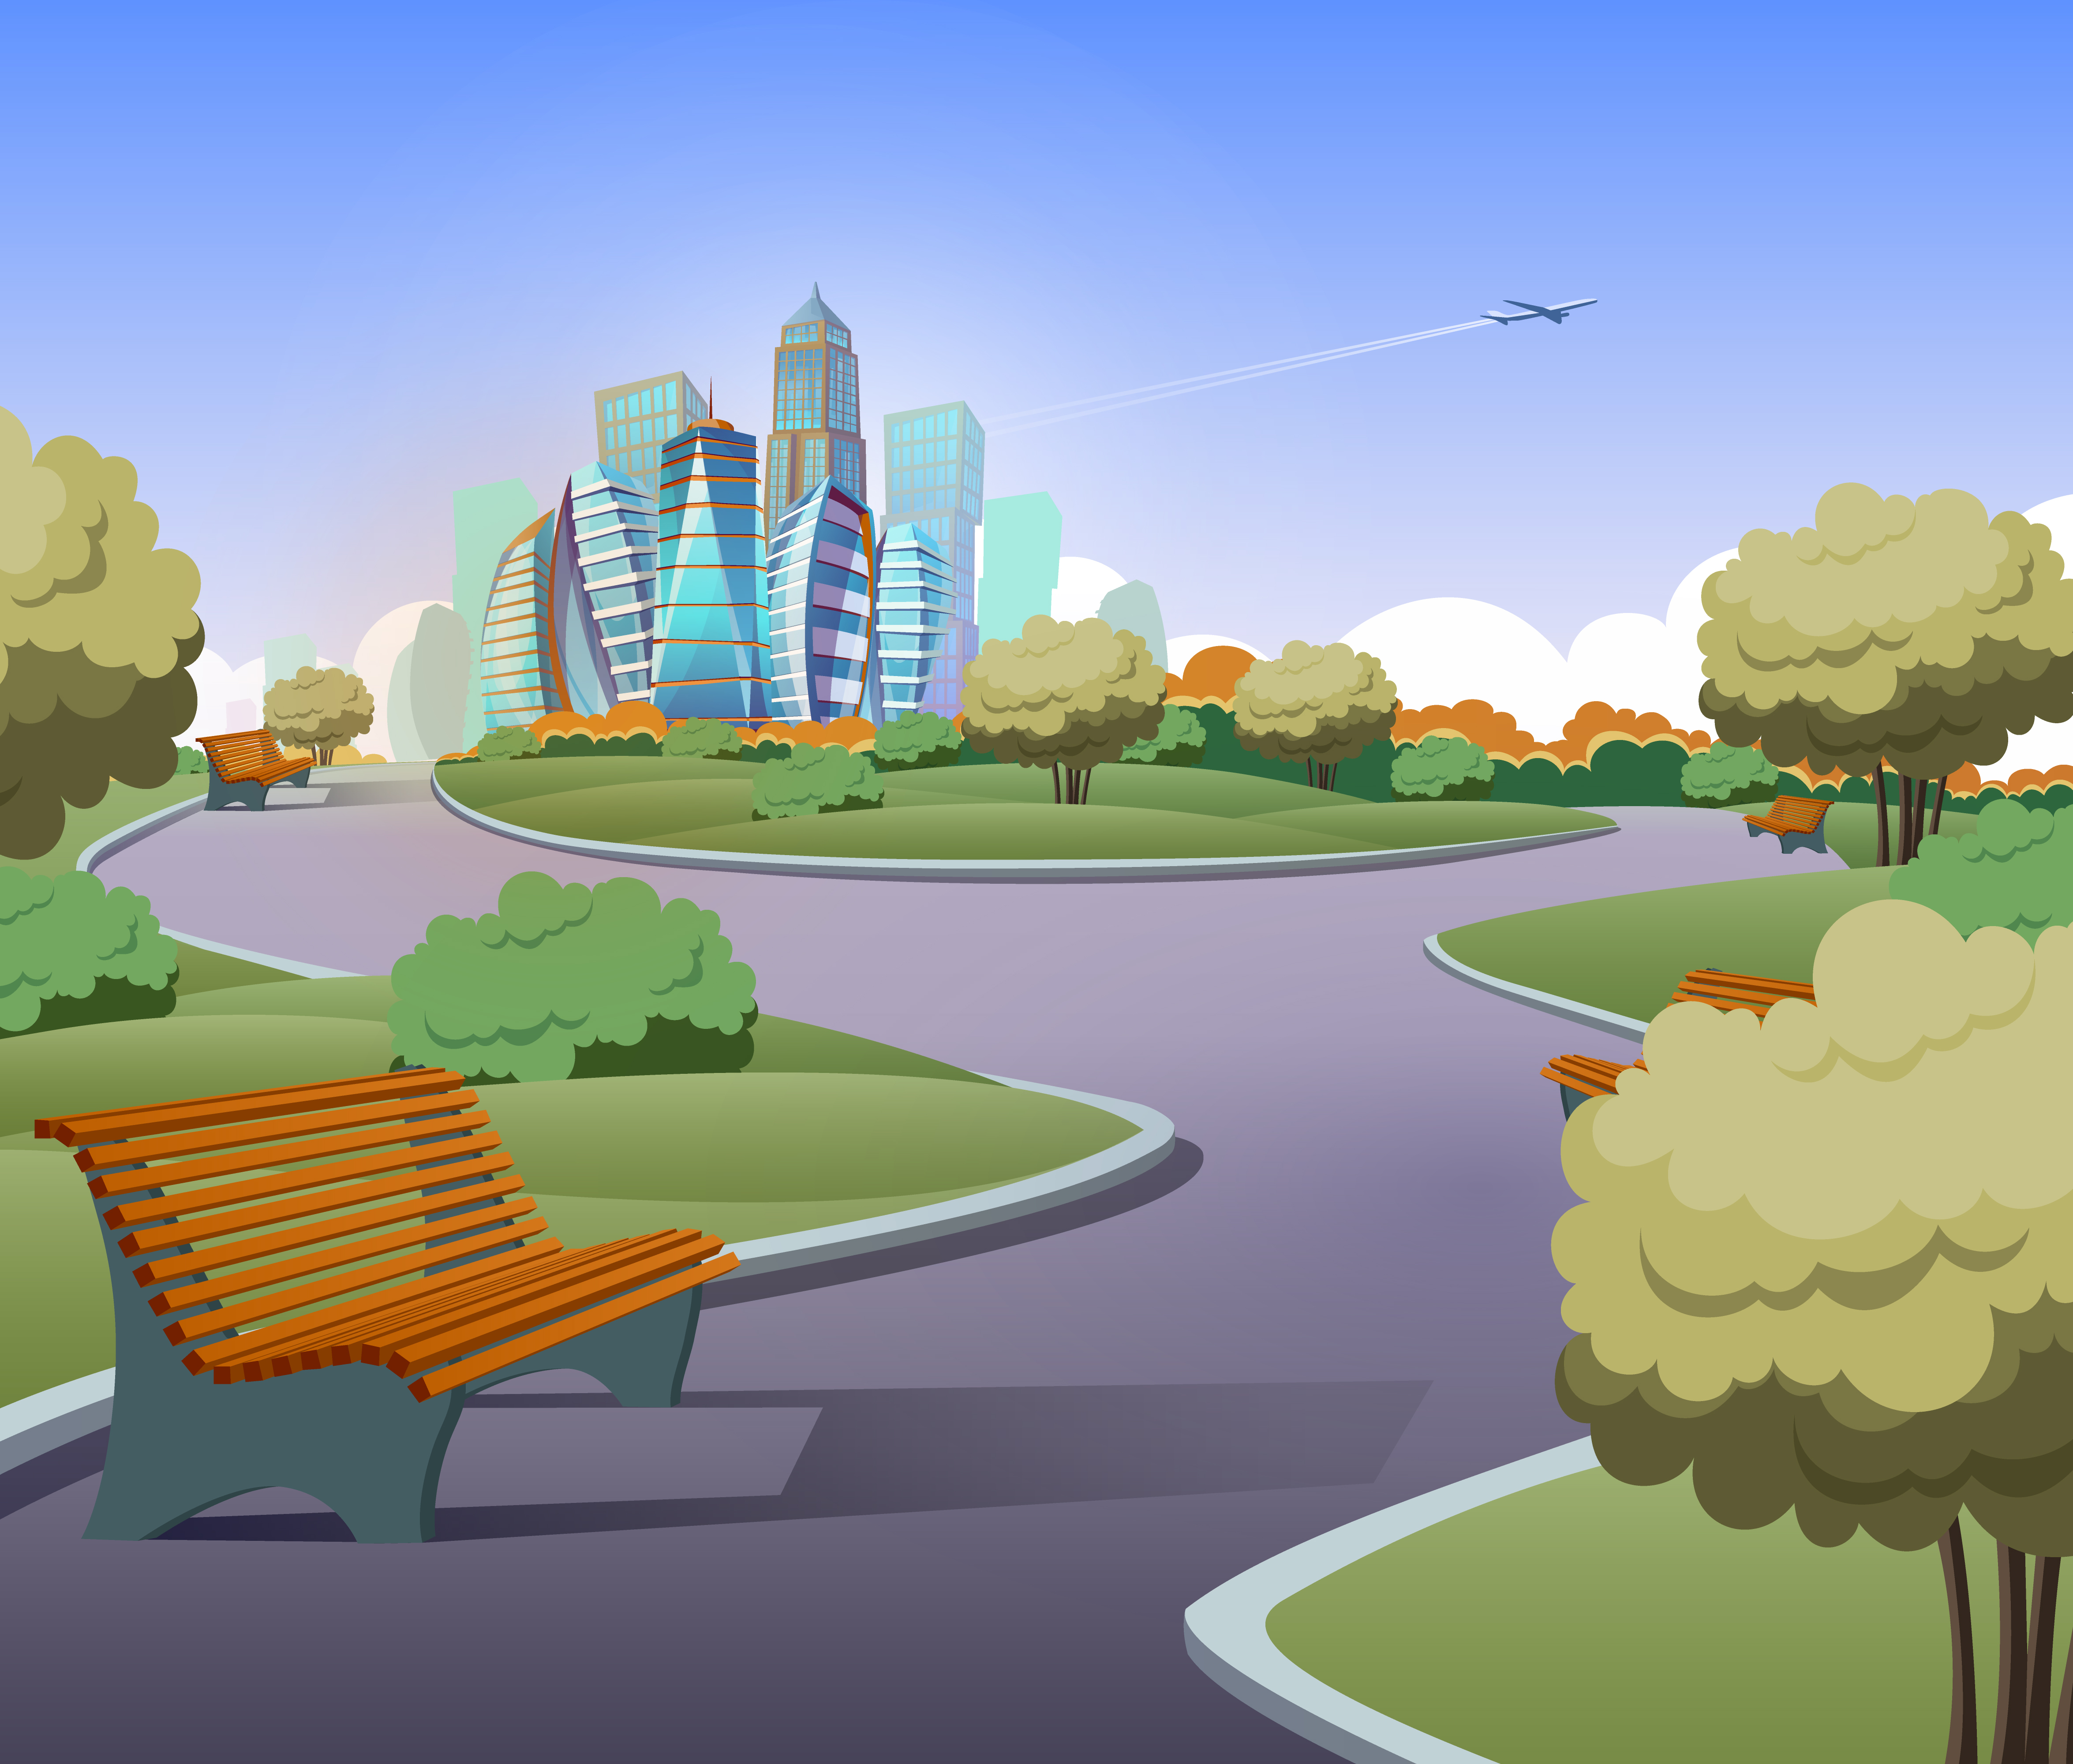
\includegraphics[width=0.5\textwidth]{./media/image62a.jpeg}
\end{center}
\vspace{1em}

De acordo com o prefeito da cidade, a nova praça é um importante espaço de lazer para a cidade. ``Estamos investindo em espaços públicos de qualidade para a população, que poderá desfrutar de um ambiente agradável e seguro para passear, praticar atividades físicas e aproveitar o tempo livre'', afirmou ele.

A obra está prevista para começar em breve e deve ser concluída em alguns meses. A prefeitura pede a colaboração da população para evitar o desperdício de água e para cuidar do novo espaço, para que todos possam desfrutar de um local agradável e bonito por muitos anos.

\fonte{Texto escrito especialmente para o material.}
\end{quote}

Lendo a notícia, pode-se concluir que a nova pista será \_\_\_\_\_\_\_ em relação à anterior.

\begin{escolha}
\begin{multicols}{2}
\item
  2 vezes maior
\item
  3 vezes maior
\item
  4 vezes maior
\item
  5 vezes maior
  \end{multicols}
\end{escolha}

